%-----------------------------------------------------------------------------------------------------------------------------------------
% MODELO DE PROJETO DE QUALIFICA��O DE MESTRADO
%
% CENTRO FEDERAL DE EDUCA��O TECNOL�GICA DE MINAS GERAIS | CEFET-MG
% DEPARTAMENTO DE PESQUISA E P�S-GRADUA��O | DPPG
% AUTOR: LINHA DE PESQUISA EM MODELAGEM, APERFEI�OAMENTO E OTIMIZA��O DE PROCESSOS | MAOP
%
% PARTE: PRINCIPAL
%
% ALUNO: Alexandre Frias Faria
%-----------------------------------------------------------------------------------------------------------------------------------------

\documentclass[12pt,a4paper]{relas}
\usepackage[brazilian]{babel}
\usepackage[T1]{fontenc}
\usepackage{epsf}
\usepackage{graphicx,color}
\usepackage{enumerate}
\usepackage{amsmath}
\usepackage{amssymb,amsmath}
\usepackage{amsfonts,latexsym,psfrag,subeqnarray,subfig}
\usepackage[latin1]{inputenc}
\usepackage{lscape}
\usepackage[round]{natbib}
\usepackage{bibentry}
\usepackage{verbatim}
\usepackage{multirow}
\usepackage{makeidx}
\usepackage{booktabs}
\usepackage{slashbox}
\usepackage{scalefnt}
\usepackage{indentfirst}
\usepackage{natbib}
%\makeindex

\setlength{\bibhang}{0pt}
\let\cite\citep
% apaguei as chaves do algorithm2e em espanhol no algoritmo.sty
% \usepackage[portuguese,ruled,lined]{algorithm2e}
\usepackage[portuguese,ruled,lined]{algoritmo}
\setcounter{secnumdepth}{5}
\setcounter{tocdepth}{2}

\textwidth=15cm
\textheight= 24cm
\topmargin= 0.16cm
\headheight=0cm
\oddsidemargin= 2.5cm
\usepackage[breaklinks=true, pdftoolbar=true, pdfmenubar=true]{hyperref}
\hypersetup{
    colorlinks,
    citecolor=blue,
    filecolor=black,
    linkcolor=blue,
    urlcolor=black
}

\usepackage{breakurl}

\usepackage[normalem]{ulem}



%------------------------------comandos para enunciar e enumerar enunciados
\newcommand{\dem}{\quad {\bf Demonstra��o:}\quad}
%\newcommand{\fim}{\newline \begin{flushright} $\blacksquare$ \end{flushright}}
\newcommand{\fim}{\null \hfill \mbox{$\Box$}}
\newtheorem{defi}{Defini��o}[section]
\newtheorem{lema}{Lema}[section]
\newtheorem{conj}{Conjectura}[section]
\newtheorem{perg}{Pergunta}[section]
\newtheorem{exem}{Exemplo}[section]
\newenvironment{prova}{\noindent {\bf Prova:}}{\hfill $\Box$ \\}
\newtheorem{axi}{Axioma}[section]
\newtheorem{prop}{Propriedade}[section]
\newtheorem{obs}{Observa��o}[section]
\newtheorem{teo}{Teorema}[section]
\newtheorem{corol}{Corol�rio}[section]
\newtheorem{res}{Resolu��o}[section]
%------------------------------------------------------------------------------


\newcommand\vi{\vspace{\baselineskip}}
\newcommand\hi{\hspace*{\parindent}}

\begin{document}

%-----------------------------------------------------------------------------------------------------------------------------------------
% PR�-TEXTUAIS
%-----------------------------------------------------------------------------------------------------------------------------------------

%-----------------------------------------------------------------------------------------------------------------------------------------
% MODELO DE PROJETO DE QUALIFICA��O DE MESTRADO
%
% CENTRO FEDERAL DE EDUCA��O TECNOL�GICA DE MINAS GERAIS | CEFET-MG
% DEPARTAMENTO DE PESQUISA E P�S-GRADUA��O | DPPG
% AUTOR: LINHA DE PESQUISA EM MODELAGEM, APERFEI�OAMENTO E OTIMIZA��O DE PROCESSOS | MAOP
%
% PARTE: FOLHA DE ROSTO
%
% ALUNO: Alexandre Frias Faria
%-----------------------------------------------------------------------------------------------------------------------------------------

\pagenumbering{roman} \hoffset -20mm
\thispagestyle{empty} \null \vskip -1cm
\begin{tabular}[t]{ll}
    \hspace{-1.2cm}
    \begin{minipage}[bl]{4.5 cm}
        \includegraphics*[width=3.5cm,height=2.44cm]{logoCefet}
    \end{minipage} &
        \hspace{-1.6cm}
    \begin{minipage}[tl]{9cm}
        \begin{tabular}[t]{l}
            {\Large \bf CENTRO FEDERAL DE EDUCA��O} \\
            {\Large \bf TECNOL�GICA DE MINAS GERAIS}
            \vspace{0.2cm} \\
            {\large \bf Diretoria de Pesquisa e P�s-Gradua��o}
            \vspace{0.2cm} \\
            {\large \bf Programa de P�s-Gradua��o em }\\
            {\large \bf Modelagem Matem�tica e Computacional}
       \end{tabular}
    \end{minipage}
\end{tabular}

\vspace{20mm}

%-----------------------------------------------------------------------------------------------------------------------------------------
% T�TULO
%-----------------------------------------------------------------------------------------------------------------------------------------

\begin{center}
\begin{Huge}\textsc{
\textbf{Algoritmos e Modelos \\ Matem�ticos para o Problema da \\ \vspace{2mm} k-Parti��o de N�meros}}
\end{Huge}
\end{center}

\vspace{15mm}

%-----------------------------------------------------------------------------------------------------------------------------------------
% DESCRI��O
%-----------------------------------------------------------------------------------------------------------------------------------------

\begin{flushright}
\begin{minipage}[tl]{9cm}
Projeto de Disserta��o de Mestrado, submetido ao Programa de P�s-Gradua��o em Modelagem Matem�tica e Computacional, como parte dos requisitos exigidos para a obten��o do t�tulo de Mestre em Modelagem Matem�tica e Computacional.
\end{minipage}
\end{flushright}

\vspace{10mm}

%-----------------------------------------------------------------------------------------------------------------------------------------
% AUTORES
%-----------------------------------------------------------------------------------------------------------------------------------------

\begin{flushright}
\begin{minipage}[tl]{12.5cm}
 \begin{description}
    \item[Aluno]: Alexandre Frias Faria
    \item[Orientador]: Prof. Dr. S�rgio Ricardo de Souza
    \item[Co-Orientador]: Prof. Dr. Carlos Alexandre Silva
\end{description}
\end{minipage}
\end{flushright}

%-----------------------------------------------------------------------------------------------------------------------------------------
% DATA
%-----------------------------------------------------------------------------------------------------------------------------------------

\vfill \vspace{10mm}
\begin{center}
Belo Horizonte\\
Fevereiro de 2016
\end{center}
\newpage 
%-----------------------------------------------------------------------------------------------------------------------------------------
% MODELO DE PROJETO DE QUALIFICA��O DE MESTRADO
%
% CENTRO FEDERAL DE EDUCA��O TECNOL�GICA DE MINAS GERAIS | CEFET-MG
% DEPARTAMENTO DE PESQUISA E P�S-GRADUA��O | DPPG
% AUTOR: LINHA DE PESQUISA EM MODELAGEM, APERFEI�OAMENTO E OTIMIZA��O DE PROCESSOS | MAOP
%
% PARTE: RESUMO
%
% ALUNO: Alexandre Frias Faria
%-----------------------------------------------------------------------------------------------------------------------------------------

\chapter*{\textbf{Resumo}}\label{Resumo}

\noindent
Este projeto de disserta��o de mestrado apresenta formula��o matem�tica e algoritmos para a vers�o de otimiza��o do Problema da k-Parti��o de N�meros. Este problema consiste em distribuir os elementos de um conjunto dado em $k$ subconjuntos disjuntos, de modo que as somas dos elementos de cada subconjunto fiquem no menor intervalo poss�vel. O primeiro m�todo consiste em aplicar a meta-heur�stica ILS (\emph{Iterated Local Search}) na solu��o gerada por um algoritmo aproximado. A estrat�gia � aplicar m�todo guloso em todas as fases do algoritmo, tanto na inicializa��o quanto para a escolha de movimentos do ILS. Outras propostas visam substituir o Or�culo do Algoritmo \ref{algoritmo1} pelo melhor resultado de um conjunto de heur�sticas. Por fim, o uso de algoritmos exatos para problemas relacionados, como o Problema da Soma de Subconjunto, s�o adaptados ao tema desse trabalho. Alguns resultados parciais j� publicados encontram-se no final do texto.

\vspace{0.5cm}



\noindent
\underline{PALAVRAS-CHAVE}: Problema da k-Parti��o de N�meros, Problema da Parti��o de N�meros, \emph{Iterated Local Search},  \emph{Complete Karmarkar-Karp Algorithm}.
\bigskip 
%-----------------------------------------------------------------------------------------------------------------------------------------
% MODELO DE PROJETO DE QUALIFICA��O DE MESTRADO
%
% CENTRO FEDERAL DE EDUCA��O TECNOL�GICA DE MINAS GERAIS | CEFET-MG
% DEPARTAMENTO DE PESQUISA E P�S-GRADUA��O | DPPG
% AUTOR: LINHA DE PESQUISA EM MODELAGEM, APERFEI�OAMENTO E OTIMIZA��O DE PROCESSOS | MAOP
%
% PARTE: SUM�RIO
%
% ALUNO: Alexandre Frias Faria
%-----------------------------------------------------------------------------------------------------------------------------------------

\tableofcontents
\newpage
\listoftables
\newpage
\listoffigures
\newpage 

\pagenumbering{arabic}
\pagestyle{meucabe}

%-----------------------------------------------------------------------------------------------------------------------------------------
% TEXTUAIS
%-----------------------------------------------------------------------------------------------------------------------------------------

%-----------------------------------------------------------------------------------------------------------------------------------------
% MODELO DE PROJETO DE QUALIFICA��O DE MESTRADO
%
% CENTRO FEDERAL DE EDUCA��O TECNOL�GICA DE MINAS GERAIS | CEFET-MG
% DEPARTAMENTO DE PESQUISA E P�S-GRADUA��O | DPPG
% AUTOR: LINHA DE PESQUISA EM MODELAGEM, APERFEI�OAMENTO E OTIMIZA��O DE PROCESSOS | MAOP
%
% PARTE: INTRODU��O
%
% ALUNO: Alexandre Frias Faria
%-----------------------------------------------------------------------------------------------------------------------------------------

\chapter{Introdu��o} \label{introducao}
\markboth{Introdu��o}{Introdu��o}


Entende-se por parti��o de um conjunto $S$ a uma cole��o de subconjuntos, dois a dois disjuntos, cuja uni�o forma $S$. Uma k-parti��o ocorre quando a parti��o tem exatamente $k$ subconjuntos n�o vazios. Durante o decorrer do texto, os subconjuntos pertencentes � parti��o s�o denominados de partes.

O Problema da Parti��o de N�meros (\emph{Two-Way Number Partitioning Problem} -- TWNPP) j� foi chamado de ``\emph{O mais f�cil problema NP-completo}'' por \citet{hayes:2002}, mas os problemas generalizados que derivam dele s�o muito mais complicados. Varia��es menos gerais desse problema se limitam a encontrar uma parti��o com partes de tamanho fixo, como o {\em 3-Partition Problem}, encontrado em \citet{joosten:2013}, ou mudam o objetivo original para um problema de escalonamento, como em \citet{moffitt:2013}.

Embora seja um dos 21 problemas de classe NP-completos discutidos por  \citet{karp:1972}, existem algoritmos exatos para o TWNPP, como em \citet{schroeppel:1981}, \citet{horowitz:1974} e \citet{korf:1998}), como tamb�m muitos algoritmos aproximados aplic�veis  ao problema analisados em \citet{gent:1998} e \citet{kann:2003}.




\section{Apresenta��o Inicial} \label{apres}
\markboth{Apresenta��o Inicial}{Apresenta��o Inicial}

%=======================================\cite{elon:2004}
Os conceitos de norma, di�metro e bola s�o importantes para melhor compreens�o da Se��o \ref{apres} pois com eles � poss�vel enunciar todos os problemas das Subse��es \ref{npp}, \ref{mwnpp}, \ref{mdtwnpp} e \ref{mdmwnpp} mantendo a mesma natureza da fun��o objetivo. Esses conceitos podem se encontram formalmente descritos em \cite{elon:2004}. 

\begin{defi}
Uma fun��o $\left\|.\right\|_p :\mathbb{R}^n \to \mathbb{R}^{+}$ � uma norma de $\mathbb{R}^n$ se para quaisquer $x,y\in\mathbb{R}^n$ e $a\in\mathbb{R}$:
\begin{itemize}
	\item $\left\|x\right\|_p=0\Rightarrow x=\vec{0}$
	\item $\left\|a.x\right\|_p = |a|.\left\|x\right\|_p$
	\item $\left\|x+y\right\|_p\leq \left\|x\right\|_p +\left\|y\right\|_p$
\end{itemize}\fim
\end{defi}

Nesse texto usa-se $p\to \infty$, ou seja, a norma do m�ximo que retorna a maior coordenada do vetor.


\begin{defi}
Dados dois vetores $x,y\in\mathbb{R}^n$. A dist�ncia ente $x$ e $y$ � dada por $d(x,y)=\left\|x-y\right\|_p$.\fim
\end{defi}

\begin{defi}
Dado um subconjunto $X\subset\mathbb{R}^n$. O di�metro de $X$ �  $diam(X)=\max_{x_1,x_2\in X}\{d(x_1, x_2)\}$.\fim
\end{defi}

\begin{defi}
Dado um ponto $v_0\in\mathbb{R}^n$ e um n�mero real positivo $r$. Uma bola de cetro $v_0$ e raio $r$ � o conjunto de pontos $v\in\mathbb{R}^n$ tais que $\left\|x-x_0\right\|_p \leq r$.\fim
\end{defi}

O di�metro de um conjunto � duas vezes o raio da menor bola que cont�m todos os elementos deste conjunto.

%======================================================

Com o objetivo de apresentar o Problema da k-Parti��o de N�meros, nesta se��o mostra-se uma sequ�ncia de outros problemas diretamente relacionados com o mesmo. Nota-se que � poss�vel enunciar, genericamente, todos os problemas abaixo da seguinte forma:

\begin{defi}\label{geralnpp}
Dado um conjunto $S$ de $n$ vetores $v \in \mathbb{Z}_{+}^m$ e um inteiro $k$, o objetivo � encontrar uma parti��o de $S$ com dimens�o $k$,  de modo que as somas dos elementos de cada parte fiquem contidas dentro da menor bola poss�vel. Assim, espera-se minimizar o o raio dessa bola (o di�metro do conjunto)\fim
\end{defi}



Em seguida, mostra-se um enunciado com exemplo para cada vers�o abaixo.

\subsection{Problema da Parti��o de N�meros}\label{npp}

O Problema da Parti��o de N�meros (\emph{Two-Way Number Partitioning Problem} -- TWNPP) � a tarefa de minimizar a diferen�a das somas de dois subconjuntos disjuntos de um conjunto $S$. Essa � a vers�o mais simples e popular do problema apresentada por \citet{karp:1972} e tratada em diversos artigos, como \citet{pedroso:2010} e \citet{gent:1998}. O tamanho da bola, nesse caso, � o comprimento do intervalo formado pelo resultado das duas somas. O exemplo \ref{ex1} mostra essa situa��o.

\begin{exem} \label{ex1}
O conjunto $S=\{87, 6, 5, 45, 34, 2, 24, 12, 7, 6, 54, 34\}$ pode ser particionado em:

\[
\underbrace{\{87, 34, 24, 6, 5\}}_{soma=156},\underbrace{\{54, 45, 34, 12, 7, 6, 2\}}_{soma=160}
\] 

O valor da fun��o objetivo dessa parti��o � $160-156=4$, mas a parti��o �tima �
\[
\underbrace{\{87, 34, 24, 6, 5, 2\}}_{soma=158},\underbrace{\{54, 45, 34, 12,  7, 6\}}_{soma=158}
\] 

\noindent com valor de fun��o objetivo $158-158=0$.\fim

\end{exem}

O enunciado matem�tico do Problema da Parti��o de N�meros consiste em encontrar um conjunto $A\neq\emptyset$ que minimize a fun��o:

\begin{equation}
f(A)=\left|\sum_{x\in A}x - \sum_{x\in S\setminus A}x\right| \label{eq1}
\end{equation}

A partir desse problema, encontram-se duas generaliza��es distintas, abordadas nos t�picos a seguir.

\subsection{Problema da k-Parti��o de N�meros}\label{mwnpp}

Esta primeira generaliza��o do TWNPP � o Problema da k-Parti��o de N�meros (\emph{Multi-way Number Partitioning Problem} -- MWNPP), que expande o n�mero de subconjuntos nos quais se pretende distribuir o conjunto $S$.

Dado um conjunto num�rico $S$, o objetivo � encontrar uma parti��o de dimens�o $k$, de modo que as somas dos elementos de cada parte sejam as mais pr�ximas poss�veis umas das outras. Isso se resume a ter a parte de maior soma  se aproximando da parte de menor soma tanto quanto for poss�vel. Os textos que abordam essa vers�o s�o, dentre outros, \citet{karmarkar:1982}, \citet{korf:2009}, \citet{korf:2013}. Um trabalho recente de forte interesse, pela sua completude, �  \citet{schreiber:2014}. 

O exemplo a seguir mostra uma situa��o desse problema.

\begin{exem} \label{exe11}
O conjunto $S=\{87, 6, 5, 45, 34, 2, 24, 12, 7, 6, 54, 34\}$ pode ser particionado para $k=3$ em:

\[
\underbrace{\{87,12,6\}}_{soma=105}, ~\underbrace{\{45,34,6,24\}}_{soma=109}, ~\underbrace{\{5,7,2,54,34\}}_{soma=102}
\] 
O valor da fun��o objetivo dessa parti��o � $109-102=7$, mas a parti��o �tima �
\[
\underbrace{\{87,12,6\}}_{soma=105}, ~\underbrace{\{45,34,2,24\}}_{soma=105}, ~\underbrace{\{5,7,6,54,34\}}_{soma=106}
\] 
\noindent com valor de fun��o objetivo $106-105=1$. Observe que as partes possuem dimens�es (n�mero de elementos) diferentes. \fim
\end{exem}

A entrada � um conjunto $S$ e um inteiro positivo $k$ e a sa�da � uma parti��o de $S$, na forma $\{A_1, A_2, ..., A_k\}$. O objetivo � minimizar a fun��o:
\begin{equation}
f(\{A_1, A_2, ..., A_k\})=\max_{i} \left\{ \sum_{x\in A_i}x \right\} - \min_{j} \left\{ \sum_{x\in A_j}x \right\} \label{eq2}
\end{equation}

A fun��o \ref{eq2} � uma vers�o simplificada do di�metro de um conjunto com $k$ n�meros reais $\displaystyle\sum_{x\in A_j}x$ mostrada abaixo.

\begin{equation}
f(\{A_1, A_2, ..., A_k\})=\max_{(i,j)} \left\{ \sum_{x\in A_i}x - \sum_{x\in A_j}x \right\} \label{eq0}
\end{equation}



\subsection{Problema Multidimensional da Parti��o de N�meros}\label{mdtwnpp}

A segunda generaliza��o do (TWNPP) � o Problema Multidimensional da Parti��o de N�meros  (\emph{Multidimensional Two-Way Number Partitioning Pro\-blem} -- MDTWNPP). Este problema transforma um conjunto $S$ de inteiros  em um conjunto de vetores inteiros $S=\{v_i\in \mathbb{Z}^{m}_{+}:\quad \forall i \in\{1,2,3,...,n\}\}$. Para definir este problema, faz-se necess�rio o uso de uma norma em $\mathbb{R}^{m}$.

Seu enunciado matem�tico, proposto por \citet{kojic:2010}, � muito parecido com o (TWNPP), por�m, ap�s somar os elementos de cada um dos subconjuntos, tem-se um vetor, cuja norma ser� o valor do objetivo. A busca � um conjunto $A\neq\emptyset$ que minimize a fun��o:

\begin{equation}
f(A)=\left\|\sum_{x\in A}x - \sum_{x\in S\setminus A}x \right\|_{p}
\label{eq32}
\end{equation}

Quando $p\to\infty$, a fun��o $f(\cdot)$ retorna a maior coordenada do vetor $\displaystyle\sum_{x\in A}x - \displaystyle\sum_{x\in S\setminus A}x$ sendo equivalente a fun��o objetivo do artigo citado.

Seja $ v\in \mathbb{Z}_{+}^m$ e $v_{ij}$ com $i$ indexando o vetor $v$ variando de $1$ at� $n$ e $j$ sendo a coordenada do vetor $v$ e vai de $1$ at� $m$. O conjunto $I_n$ � o conjunto dos �ndices $i$ e a vari�vel de decis�o $B$ � um subconjunto de $I_n$.

\begin{equation}
f(B)=\max_{j} \left\{ \sum_{i\in I_n\setminus B}v_{ij} - \sum_{i\in B}v_{ij} \right\} \label{eq}
\end{equation}

\begin{exem}
O conjunto
\[
\begin{array}{l}
S=\left\{ (8,3,6,3),(8,3,12,3),(8,3,0,3),(17,5,10,5),(10,5,10,5), \right. \\
~~~~~~~~~~~~~~~~~~~~~~~~~~~~~~~~~~~~~~~~~~~~\left. (10,5,10,3),(8,3,6,1),(5,3,6,3) \right\}
\end{array}
\]
\noindent  com $m=4$ e $k=2$ tem pode ser particionado como:

\[
\begin{array}{rcl}
A_1 & = & \underbrace{\{(17,5,10,5),(8,3,0,3),(10,5,10,5),(10,5,10,3)\}}_{soma=(45,18,30,16)},\\ \\
A_2 & = & \underbrace{\{(8,3,6,3),(8,3,12,3),(8,3,6,1),(5,3,6,3)\}}_{soma=(29,12,30,10)}
\end{array}
\]
\noindent com um valor de fun��o objetivo $\max\{|(45,18,30,16)-(29,12,30,10)|\}=\max\{|(16,6,0,6)|\}=16$, mas tem parti��o �tima
\[
\begin{array}{rcl}
A_1 & = & \underbrace{\{(17,5,10,5),(10,5,10,5),(10,5,10,3)\}}_{soma=(37,15,30,13)},\\ \\
A_2 & = & \underbrace{\{(8,3,6,3),(8,3,12,3),(8,3,0,3),(8,3,6,1),(5,3,6,3)\}}_{soma=(37,15,30,13)}
\end{array}
\]
\noindent com valor de fun��o objetivo $\max\{|(37,15,30,13)-(37,15,30,13)|\}=\max\{|(0,0,0,0)|\}=0$\fim
\end{exem}


\subsection{Problema Multidimensional da k-Parti��o de N�meros}\label{mdmwnpp}

O Problema Multidimensional da k-Parti��o de N�meros (\emph{Multidimensional Multi-Way Number Partitioning Problem} -- MDMWNPP � uma generaliza��o tanto do (MWNPP) quanto do (MDTWNPP). Neste problema, um conjunto de vetores de $\mathbb{Z}^{m}_{+}$ deve ser dividido em $k$ conjuntos, de modo que o di�metro desses $k$ vetores resultantes seja o menor poss�vel. O exemplo \ref{exx} ilustra essa situa��o.

\begin{exem} \label{exx}
Seja o conjunto:
\[
\begin{array}{ccl}
S & = & \left\{(37,15,30,13),(8,3,6,3),(8,3,12,3),(8,3,0,3),(17,5,10,5), \right. \\
  & & ~~~~~~~~~~~~~~~~~~~~~~~~~~\left. (10,5,10,5),(10,5,10,3),(8,3,6,1),(5,3,6,3) \right\}
\end{array}
\]
\noindent Para $m=4$ e $k=3$, pode ser particionado em:

\[
\begin{array}{rcl}
A_1 & = & \underbrace{\{(17,5,10,5),(10,5,10,5),(10,5,10,3)\}}_{soma=(37,15,30,13)},\\ \\
A_2 & = & \underbrace{\{(37,15,30,13), (8,3,0,3)\}}_{soma=(45,18,30,16)},\\ \\
A_3 & = & \underbrace{\{(8,3,6,3),(8,3,12,3),(8,3,6,1),(5,3,6,3)\}}_{soma=(29,12,30,10)}
\end{array}
\]

\noindent com valor de fun��o objetivo:
\[
\begin{array}{ccl}
\max\{|(45,18,30,16)-(29,12,30,10)|, |(37,15,30,13)-(29,12,30,10)|,\\ |(45,18,30,16)-(37,15,30,13)|\}=\max\{|(16,6,0,6)|, |(8,3,0,3)|, |(8,3,0,3)|\}=16
\end{array}
\]
\noindent mas com parti��o �tima:
\[
\begin{array}{rcl}
A_1 & = & \underbrace{\{(17,5,10,5),(10,5,10,5),(10,5,10,3)\}}_{soma=(37,15,30,13)},\\ \\
A_2 & = & \underbrace{\{(37,15,30,13)\}}_{soma=(37,15,30,13)},\\ \\
A_3 & = & \underbrace{\{(8,3,6,3),(8,3,12,3),(8,3,0,3),(8,3,6,1),(5,3,6,3)\}}_{soma=(37,15,30,13)}
\end{array}
\]
\noindent com valor de fun��o objetivo igual a $0$ pois todas as partes tem igual soma. Sendo assim o di�metro desse conjunto � a maior coordenada de $3$ vetores nulos.\fim
\end{exem}

Ou seja, o objetivo � equivalente a minimizar a maior dist�ncia entre dois de todos os vetores, dada pela express�o:

\begin{equation}
f(\{A_1,A_2,...,A_k\}) = \max_{(i,j)} \left\{ \left\| \sum_{x \in A_i} x  - \sum_{x \in A_j} x \right\|_p \right\}
\label{eq31}
\end{equation}

A express�o (\ref{eq31}) pode ser utilizada como a fun��o objetivo de qualquer um dos problemas enunciados acima, seja do Problema apresentado na Se��o \ref{npp}, seja do Problema apresentado na Se��o \ref{mdmwnpp} atual, sem qualquer inconsist�ncia.

O trabalho de \citet{petrica:2013} adapta um outro modelo para o MDMWNPP, a partir da formula��o matem�tica apresentada em \citet{kojic:2010} para o MDTWNPP mostrado na Subse��o \ref{mdtwnpp}.

Seja $ v_i \in \mathbb{Z}_{+}^m$ e $ V_l=\displaystyle\sum_{v_i\in A_l}v_i $. A fun��o objetivo � a maior diferen�a entre duas coordenadas de $V_{l_1}$ e $V_{l_2}$ com $l_1\neq l_2$, na forma:

\begin{equation}
f(\{A_1,A_2,...,A_k\})=\max_{j}\left\{ \left| \max_{l} \sum_{i\in A_l} v_{ij} - \min_{l} \sum_{i\in A_l} v_{ij} \right| \right\} \label{eq3}
\end{equation}
Nesta express�o, $l$ indexa as partes e vai de $1$ at� $k$; $i$ vai de $1$ at� $n$ e indexa o vetor $v$ dentro da parte $A_l$; $j$ � a coordenada do vetor $v$ e vai de $1$ at� $m$.

Note que, ao contr�rio de todos os enunciados at� aqui, a express�o (\ref{eq3}) n�o � igual � express�o (\ref{eq31}) quando $p\to\infty$. Esta formula��o est� fora do padr�o da Defini��o \ref{geralnpp}.


A Figura \ref{figura1} resume as rela��es entre os quatro problemas apresentados.

\begin{figure}[!h]
\centering
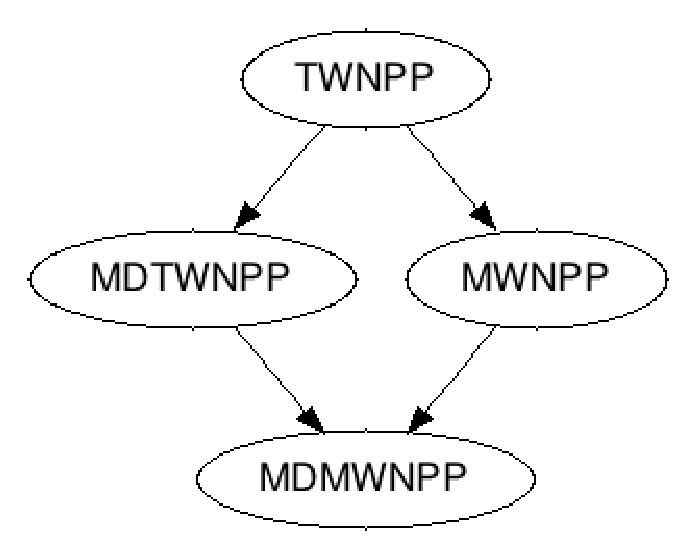
\includegraphics[width=0.4\linewidth]{chart}
\caption{Rela��es entre os 4 problemas.}
\label{figura1}
\end{figure}

%\newpage
\section{Organiza��o do Projeto}
\markboth{Organiza��o do Projeto}{Organiza��o do Projeto}

O restante do texto est� organizado segundo os coment�rios em cada cap�tulo a seguir. No Cap�tulo \ref{problema}, mostra-se o problema tratado com uma vis�o mais detalhada, usando enunciado, modelo matem�tico proposto e uma vis�o mais te�rica sobre como encontrar suas solu��es. O Cap�tulo \ref{teorica} cont�m algoritmos para problemas auxiliares aos m�todos propostos do Cap�tulo \ref{algoritmos}. O Cap�tulo \ref{revisao} cont�m um hist�rico de trabalhos sobre temas relacionados ao mesmo problema tratado nesse texto. O Cap�tulo \ref{algoritmos} apresenta algoritmos propostos j� implementados e testados, junto com poss�veis abordagens ainda n�o definitivas. Apresenta-se o que � esperado para as propostas desse trabalho no Cap�tulo \ref{objetivo}. Um conjunto de metas at� a defesa da disserta��o est� no Capitulo \ref{cronograma}. Os resultados do Cap�tulo \ref{resultados} s�o preliminares e se encontram publicados.



\chapter{Caracteriza��o do Problema} \label{problema}
\markboth{Caracteriza��o do Problema}{Caracteriza��o do Problema}

Este cap�tulo apresenta o problema abordado neste projeto de disserta��o. Est� organizado da seguinte forma: a Se��o \ref{definicao} apresenta a defini��o do problema e discute sua dificuldade combinat�ria. A Se��o \ref{formulacao} introduz uma formula��o matem�tica para o problema em Otimiza��o Linear Inteira. A Se��o \ref{avaliacao} mostra uma solu��o te�rica exata. 

\section{Defini��o} \label{definicao}

O Problema da k-Parti��o de N�meros (\emph{Multi-Way Number Partitioning Problem} -- MWNPP apresentado na Se��o \ref{mwnpp} � a vers�o abordada, originalmente, em \citet{karmarkar:1982}. Sua entrada � um conjunto $S$ e a sa�da � uma parti��o de $S$ com tamanho $k$.

\begin{defi}
Seja $S=\{a_1,a_2, ..., a_n\}$ um conjunto de inteiros positivos $a_l$, $l = 1, \ldots, n$, e $k$ um n�mero inteiro positivo. O Problema da k-Parti��o de N�meros consiste em encontrar uma k-parti��o de $S$, na forma $\{A_1, A_2, ..., A_k\}$, que minimize a fun��o $f$ definida por:
\begin{equation}
f(\{A_1, A_2, ..., A_k\})=\max_{i}\left\{\sum_{x\in A_i}x\right\}-\min_{j}\left\{\sum_{x\in A_j}x\right\}
\end{equation} {\null \hfill \mbox{$\Box$}}
\end{defi}

A dificuldade combinat�ria desse problema, quando resolvido por uma enumera��o ing�nua das k-parti��es de $S$, � dada pelo N�mero de Stirling $S(n,k)$\footnote{\url{http://mathworld.wolfram.com/StirlingNumberoftheSecondKind.html}}, que conta a quantidade de formas distintas de se repartir um conjunto de tamanho $n$ em $k$ partes. Encontra-se uma an�lise mais detalhada do N�mero de Stirling em \citet[p�g. 80ff]{stanley:1997} e em \citet{griffiths:2010}.

Defina $S(n-1,k)$ como o n�mero de parti��es com $k$ partes de um conjunto com $n-1$ elementos. Claro que o n�mero de n-parti��es de um conjunto com $n$ elementos � $1$ (ou seja, $S(n,n)=1$) e o n�mero de 1-parti��o de qualquer conjunto � $1$ (ou seja, $S(n,1)=1$). Se um n-�simo elemento for adicionado ao conjunto, � poss�vel descobrir $S(n,k)$ usando duas informa��es: $S(n-1,k-1)$ e $S(n-1,k)$.

Inserindo o n-�simo elemento como a k-�sima parte, existem $S(n-1,k-1)$ possibilidades. Inserindo o n-�simo elemento em uma das $k$ partes j� existentes, contadas por $S(n-1,k)$, tem-se $k~S(n-1,k)$ possibilidades:

\begin{equation}
S(n,k)=S(n-1,k-1) ~+~ k~S(n-1,k) \label{exxx}
\end{equation}


\begin{exem}
Seja o conjunto de inteiros $A=\{1,2,3\}$, para $n=3$ e considere $k=2$. Assim, o N�mero de Stirling produz $S(3,2)=3$. Desse modo as parti��es s�o dadas por:
\[
\begin{array}{c}
\{1,2\},\{3\} ;\\
\{1,3\},\{2\} ;\\
\{2,3\},\{1\} ;\\
\end{array}
\]

Seja agora o mesmo conjunto de inteiros $A=\{1,2,3\}$, para $n=3$ e considere $k=1$. Assim, o n�mero de Stirling leva a $S(3,1)=1$ e � parti��o:
\[
\{1,2,3\}
\]

Considere agora o conjunto de inteiros $A=\{1,2,3,4\}$ para $n=4$ e seja $k=2$. Desse modo, as parti��es s�o:
\[
\begin{array}{c}
\{1,2,3\},\{4\} ; \{1,2\},\{3,4\} ;\\
\{1,2,4\},\{3\} ; \{1,3\},\{2,4\} ;\\
\{1,3,4\},\{2\} ; \{1,4\},\{2,3\} ;\\
\{2,3,4\},\{1\}
\end{array}
\]

Ou seja, a partir da express�o (\ref{exxx}), tem-se que:
\[
S(4,2)=S(3,1)+2.S(3,2)=7
\]{\null \hfill \mbox{$\Box$}}
\end{exem}

Al�m de enumerar todas as parti��es de tamanho $k$, ainda � justo inserir um fator multiplicador $O(n)$, respons�vel pelo custo de se avaliar a fun��o objetivo. No fim dos c�lculos, a ordem de complexidade do algoritmo ing�nuo seria $O(n.S(n,k))$.

O N�mero de Stirling n�o tem f�rmula fechada. Uma outra alternativa para expressar essa quantidade, vista em \citet{stanley:1997} � a express�o:

\begin{equation}
S(n,k)=\frac{1}{k!}\sum_{j=0}^{k}(-1)^{k-j}{k\choose j}j^{n}
\end{equation}

Esse n�mero supera as complexidades de ordem exponenciais quando o valor de $k$ segue a sequ�ncia \href{http://oeis.org/A024417}{A024417}\footnote{\url{http://oeis.org/A024417}}. Se $a(n)\in A024417$ ent�o $S(n,a(n))\geq S(n,k), \quad \forall k$. Esse fato pode ser conferido em \href{http://oeis.org/A002870}{A002870}\footnote{\url{http://oeis.org/A002870}}, a sequ�ncia do Maior N�mero de Stirling indexada em $n$. Se $a(n)\in A024417$, ent�o $S(n,a(n))\in A002870$. O gr�fico abaixo mostra casos exponenciais em escala logar�tmica comparados ao n-�simo Maior N�mero de Stirling. Este gr�fico � composto por retas sendo cortadas por uma fun��o crescente.

A { \em On-Line Encyclopedia of Integer Sequences} - OEIS � uma base de dados p�blica com variadas sequ�ncias de n�meros inteiros criada por \cite{sloane:1991}. Nela � poss�vel buscar uma sequ�ncia num�rica apenas digitando seus primeiros termos e, tamb�m, encontrar os principais artigos ligados a mesma. � a fonte das sequ�ncias \href{http://oeis.org/A002870}{A002870} e \href{http://oeis.org/A024417}{A024417}.



\begin{figure}[!h]
\centering
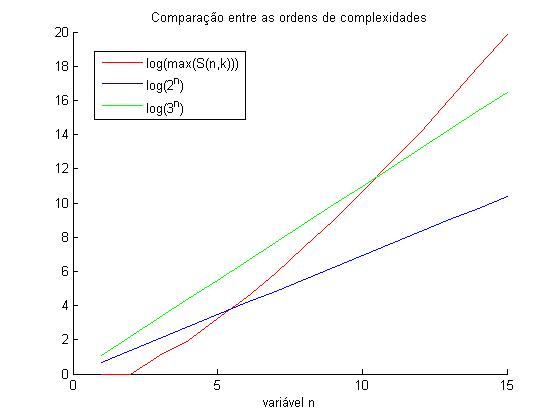
\includegraphics[width= 0.8 \linewidth]{./complex}
\caption{O maior dos N�meros de Stirling vs fun��es exponenciais. Dados retirados de \citet{sloane:1991}}
\label{figura2}
\end{figure}

Esta figura mostra que o Maior N�mero de Stirling domina assintoticamente fun��es exponenciais, ou seja, para todo $c>1$ existe um $n$ suficientemente grande tal que$S(n,a(n))>c^n$.

\section{Formula��o Matem�tica} \label{formulacao}

O modelo matem�tico de Otimiza��o Linear Inteira proposto nesse trabalho, como contribui��o efetiva, usa duas vari�veis inteiras para representar o limite inferior $t_1$ e superior $t_2$, para a soma dos elementos de todas as $k$ partes. As demais vari�veis $x_{ij}$ s�o bin�rias e informam se um elemento est� ou n�o numa parti��o. A nota��o $I_m = \{y\in\mathbb{Z}: \quad 1\leq y\leq m\}$ significa todos os inteiros entre $1$ e $m$, inclusive.


\begin{eqnarray}
\min && \label{r1} t_2 - t_1 \\
\mbox{suj. a}  &&  \label{r2} t_1 \leq \sum_{i=1}^{n}a_i x_{ij} \leq t_2, \quad \forall j\in I_k \\
&&  \label{r3} \sum_{j=1}^{k} x_{ij} =1, \quad \forall i\in I_n \\
&&  \label{r5} t_1,t_2\in\mathbb{Z_{+}} \\
&&  \label{r6} x_{ij}\in\{0,1\}
\end{eqnarray}

A rela��o de pertin�ncia (\ref{r6}) indica que $x_{ij}=1$ se o elemento de �ndice $i$ do conjunto $S$ pertence � parte de �ndice $j$. A rela��o (\ref{r5}) informa que os limitantes da maior e menor soma dos elementos das parti��es � sempre positiva. As $n$ equa��es indicadas pela express�o (\ref{r3}) garantem que as parti��es s�o disjuntas e que todos os elementos de $S$ est�o alocados em alguma parte, j� que o problema s� est� bem definido quando $n>k$. As $k$ inequa��es (\ref{r2}) mostram que o modelo garante que cada parti��o � n�o vazia, pois $t_1>0$, por efeito de (\ref{r5}) e, tamb�m, que est�o todas contidas no intervalo $[t_1, t_2]$. Por fim, a express�o (\ref{r1}) � o tamanho do intervalo que cont�m todas as $k$ somas dos elementos das partes e o objetivo de minimiza��o.

\section{Vis�o Te�rica} \label{avaliacao}

Uma abordagem mais algor�tmica do problema sugere a constru��o de um algoritmo polinomial para o (MWNPP), usando um algoritmo hipot�tico que retorna sim ($1$) ou n�o ($0$) para uma pergunta espec�fica sobre a entrada. Esse algoritmo chama-se Or�culo e � denotado por $Or(S,S')$, sendo $S$ e $S'$  duas inst�ncias de tamanho $n$ e $n-1$, respectivamente, do (MWNPP).

A pergunta em quest�o �:
\begin{perg}
As entradas $S$ e $S'$ t�m o mesmo valor �timo de fun��o objetivo~?
\end{perg}

O exemplo \ref{exemplo1} mostra uma situa��o associada ao uso desse Or�culo.

\begin{exem}\label{exemplo1}
Suponha que $k=3$, $S'=\{1,2,3,4\}$ e $S=\{1,2,3,5,6\}$. O resultado de $Or(S,S') = Or(\{1,2,3,5,6\},\{1,2,3,4\})=1$ (SIM) pois a 3-parti��o �tima de $S$ pode ser: $\{1,2,3\},\{5\},\{6\}$ ou $\{2,3\},\{1,5\},\{6\}$ ambas com valor de fun��o objetivo igual a $1$. Assim como $S'$, que tem 3-parti��o �tima $\{1,2\},\{3\},\{4\}$, com valor de fun��o objetivo igual a $1$. \fim
\end{exem}

A ideia central dessa t�cnica � decidir se dois elementos distintos do conjunto $S$ pertencem ou n�o � mesma parti��o, com a troca de dois elementos do conjunto pela soma dos mesmos. Sempre que essa troca n�o mudar o valor �timo, significa que os dois valores substitu�dos pertencem � mesma parti��o.

\begin{exem}\label{exemplo2}
Inicialmente, $S=\{1,2,3,5,6\}$. Cria-se um novo conjunto $S'=\{1+2,3,5,6\}$. Fazendo a chamada do or�culo sobre $S$ e $S'$, descobre-se que $1$ e $2$ est�o contidos na mesma parte quando $Or(S,S')=1$ e que est�o em partes distintas quando caso contr�rio. Nesse exemplo, � claro que $Or(\{1,2,3,5,6\}, \{3,3,5,6\})=1$ (veja no exemplo \ref{exemplo1}). \fim
\end{exem}



\begin{algorithm}[H] \label{algoritmo1}
\SetAlgoLined
\Entrada{$Or()$ e um conjunto $S$}
\Saida{$\{A_1, A_2, ..., A_k\}$}
\Inicio{
	$j=1$\;
	\Enqto{$S \neq \varnothing $}{
		$ k=1$\;
		$ insere(A_j, a_k)$\;
		\Para{$a_i \in S-\{a_k\}$}{
			$S'=S$\;
			$ remove(S', a_i)$\;
			$ insere(S', a_i+a_k)$\;
			\Se{$Or(S,S')=1$}{
				$ insere(A_j, a_i)$\;
				$S=S'$\;
			}
		}
		$j=j+1$\;
	}
	\Retorna{$\{A_1, A_2, ..., A_k\}$}\;
}
\caption{Algoritmo exato hipot�tico}
\end{algorithm}

O funcionamento do algoritmo � simples e direto. Primeiro, o elemento $a_1$ vai para a parte $A_1$, sendo o elemento l�der da primeira parte. Em seguida, para cada $a_i\in S-\{a_1\}$, o elemento $a_i$ � trocado por $a_1+a_i$, formando um novo conjunto $S^{i}$. Executa-se $Or(S,S^{i})$ e, sempre que a resposta do or�culo for positiva, retira-se $a_i$ de $S$, armazenando-o em $A_1$ e $S$ � trocado por $S^{i}$. Repete-se o procedimento at� $S=\varnothing$, $k-1$ vezes.

No pior caso, este algoritmo faz $O(n^2)$ chamadas ao or�culo, pois compara o elemento l�der de $A_j$ com cada um dos restantes em $S$.





\chapter{Fundamenta��o Te�rica} \label{teorica}
\markboth{Fundamenta��o Te�rica}{Fundamenta��o Te�rica}


Este Cap�tulo apresenta os fundamentos b�sicos relacionados ao tema do projeto. A Se��o \ref{graham} apresenta o Algoritmo (LPT). A Se��o \ref{interchange} mostra o Algoritmo  0/1-{\em Interchange}, ambos desenvolvidos para problemas de escalonamento de m�quinas. A Se��o {mochila} discute a rela��o do Problema da k-Parti��o de N�meros com o Problema da Mochila. A Se��o apresenta a vers�o geral da metaheur�stica \emph{Iterated Local Search} (ILS). Por fim, a Se��o \ref{karmakarp} introduz a Heur�stica de Karmarkar-Karp e sua adapta��o ao  Problema da k-Parti��o de N�meros. 


\section{Algoritmo (LPT)}\label{graham}

Proposto por \citet{graham:1966,graham:1969}, o algoritmo guloso {\em Longest Processing Time first} (LPT) foi desenvolvido para um problema de Parti��o M�nima e para o Problema de Escalonamento de Tarefaz diferente do Problema da k-Parti��o de N�meros (MWNPP), como comenta \citet{korf:2010}. 

Este algoritmo garante um resultado com raz�o de aproxima��o menor que $\frac{4}{3}-\frac{1}{3k}$ do �timo global em rela��o � fun��o objetivo $\displaystyle\max_{1\leq i\leq k}\left\{\sum_{x\in A_i}x \right\} $. Isso significa que, se $OPT(S)$ � o valor �timo da fun��o objetivo e $LPT(S)$ o valor de fun��o objetivo do LPT para uma inst�ncia $S$, a raz�o entre estes valores � tal que:
\begin{equation}\label{aproxlpt}
\frac{LPT(S)}{OPT(S)}\leq \frac{4}{3}-\frac{1}{3k}
\end{equation}
A demonstra��o de aproximabilidade se encontra em  \citet{kann:2003}.


\begin{exem} \label{exemplo3}
O resultado �timo do Problema da k-Parti��o de N�meros para a inst�ncia:
\[
S = \{8,7,6,5,4\}
\]
\noindent  e $k=2$ �
\[
\{8,7\} \quad ~~\mbox{e}~~ \quad \{6,5,4\}
\]
\noindent A parte com a maior soma � $max\{8+7, ~ 6+5+4\}=15$. Substituindo $k=2$ na desigualdade \ref{aproxlpt} tem-se $\left(\frac{4}{3}-\frac{1}{6}\right)~15=\frac{7}{6}~15=17.5$.Portanto, a resposta do algoritmo (LPT) sempre � uma parti��o em que a maior soma � menor que $17.5$ como:
\[
\{ 8, 5, 4\} \quad ~~\mbox{e}~~ \quad \{7,6\}
\]
\noindent cuja maior soma � $17$, resultado encontrado pelo (LPT), mas nunca um valor $18$ como a parti��o abaixo:
\[
\{ 8,4\} \quad ~~\mbox{e}~~ \quad \{7,6,5\}
\] {\null \hfill \mbox{$\Box$}}
\end{exem}

O algoritmo consiste em ordenar o conjunto $S$ em ordem n�o crescente e alocar os n�meros, sempre inserindo o novo elemento na parte de menor soma e, em caso de empate, desempata-se arbitrariamente. Este algoritmo tem um custo com\-pu\-ta\-cio\-nal $O(nlog(n))$ para ordenar a entrada e um custo $O(n)$ para alocar os elementos nas $k$ partes. Finalmente, a complexidade do m�todo � $O(nlog(n))$.

O Algoritmo {\em Longest Processing Time first} (LPT) est� apresentado no Algoritmo \ref{algoritmo2}. 

\begin{algorithm}[H]\label{algoritmo2}
\Entrada{Conjunto $S$ de n�meros inteiros e um inteiro k}
\Saida{Parti��o do conjunto $S$, $\{A_1, A_2, ..., A_k\}$, com tamanho k}
\Inicio{
	\Para{$j\in \{1, ..., k\}$}{
		$A_j=\emptyset$\;
		$L_j=0$\;
	}
	Ordene $S$ em ordem decrescente\;
	\Para{$a\in S$}{
		$l=\arg \min_{j} L_j$\;
		$A_l=A_l\cup a$\;
		$L_l=L_l+a$\;
	}
	\Retorna{$\{A_1, A_2, ..., A_k\}$}
}
\caption{{\em Longest Processing Time} para $k$ m�quinas}
\end{algorithm}


\section{Algoritmo 0/1-{\em Interchange}}\label{interchange}

O Algoritmo 0/1-\emph{Interchange}, proposto por \citet{horowitz:1979}, tamb�m � um m�todo para o Problema de Escalonamento em $k$ m�quinas id�nticas. Partindo de uma distribui��o inicial das tarefas, o algoritmo ordena os processadores em ordem n�o decrescente.

Seja $d_i = L(A_1) - L(A_k)$ a diferen�a entre o instante de finaliza��o do processador mais carregado e do menos carregado na itera��o $i$. Enquanto existir uma tarefa $p\in A_1 ~:~ p<d_i$, est� ser� realocada para $A_k$. Este algoritmo tem uma complexidade de tempo computacional da ordem $O(n.log(k))$, como demonstrado por \citet{langston:1982}

O Algoritmo 0/1-\emph{Interchange} est� apresentado no Algoritmo \ref{algoritmo3}.\\

\begin{algorithm}[H]\label{algoritmo3}
\Entrada{K-Parti��o $\{A_1, A_2, ..., A_k\}$ do conjunto $S$}
\Saida{K-Parti��o do conjunto $S$, $\{A_1, A_2, ..., A_k\}$}
\Inicio{
	Ordene os tempos de cada m�quina $L(A_1)\geq ...\geq L(A_k)$\;
	$d=L(A_1)-L(A_k)$\;
	\Enqto{$\exists q\in A_1 ~:~  L(q)<d$}{
		$remove(A_1, q)$\;
		$insere(A_k, q)$\;
		$L(A_1)=L(A_1)-L(q)$\;
		$L(A_k)=L(A_k)+L(q)$\;
		$d=L(A_1)-L(A_k)$\;
	}
	\Retorna{$\{A_1, A_2, ..., A_k\}$}\;
}
\caption{Algoritmo 0/1-{\em Interchange}}
\end{algorithm}


\section{Problema da Mochila/Soma de Subconjuntos}\label{mochila}

O Problema da Mochila � um dos mais estudados em Otimiza��o Combinat�ria e costuma ser um subproblema muito comum em  v�rios trabalhos. Todas as varia��es do Problema da Mochila s�o NP-completos, mas admitem uma solu��o pseudo-polinomial, como pode ser encontrado em \citet{garey:1979} e \citet{kann:2003}.

\begin{defi}
Seja $W\in\mathbb{N}$ e um conjunto de itens $I=\{1,2,...,n\}$, tal que cada elemento de $I$ indexe um peso $w_i$ e um valor $p_i$. Encontre um subconjunto de itens que maximize o valor da mochila, respeitando sua capacidade de peso, dada por $W$.\fim
\end{defi}

A formula��o matem�tica para esse problema �:

\begin{eqnarray}
\max && \sum_{j=1}^{n} p_j x_{j} \label{eq11} \\
\mbox{s.a} && \sum_{j=1}^{n}w_i x_{j}\leq W  \label{eq12} \\
&& x_{j}\in\{0,1\} \label{eq13}
\end{eqnarray}

O Problema da Soma de Subconjunto � um caso particular do Problema da Mochila, caracterizado por $\forall i\in I ~:~  w_i=p_i$. O algoritmo  pseudo-polinomial para resolve-lo tem custo $O(nW)$ e, por isso, costuma ser o mais indicado quando o conjunto de itens $I$ possui grande dimens�o, mas o n�mero $W$ tem poucos algarismos. Caso contr�rio, os algoritmos exatos mais eficientes s�o os propostos por \citet{horowitz:1974} e \citet{schroeppel:1981}. A ideia da solu��o � a seguinte:

\begin{itemize}
\item Caso o item $i$ fa�a parte da solu��o �tima considerando os itens $\{i,..., n\}$, tem-se uma solu��o com valor $p_i$ a mais do que a solu��o �tima para os itens $\{i+1,..., n\}$, com capacidade restante $W-w_i$. Esta ideia corresponde a fazer $x_i=1$, gerando o subproblema:
\begin{equation}
p_i + \max\left\{\sum_{j=i+1}^{n} p_j x_{j}~|~\sum_{j=i+1}^{n}w_j x_{j}\leq w-w_i, ~~ x_{j}\in\{0,1\}\right\}
\end{equation}
\item Caso contr�rio,  tem-se um valor correspondente � solu��o �tima para itens $\{i+1,..., n\}$ com capacidade $W$. Esta ideia corresponde a fazer $x_i=0$, gerando o subproblema
\begin{equation}
\max\left\{\sum_{j=i+1}^{n} p_j x_{j}~|~\sum_{j=i+1}^{n}w_j x_{j}\leq w, ~~ x_{j}\in\{0,1\}\right\}
\end{equation}
\end{itemize}

Assim, seja $M(i, w)$ o valor da solu��o �tima para os itens $\{i,..., n\}$ e capacidade $W$, na forma: 
\[
M(i,w)=\max\{M(i+1,w), M(i+1, w-w_i)+p_i\}
\]
\noindent e o valor �timo do problema ser� $M(1,W)$. 

O Algoritmo \ref{algoritmo4} formaliza o procedimento.

%%%%%%%%%%%%%%%
\begin{algorithm}[H]\label{algoritmo4}
\Entrada{Vetor $v$ de tamanho $n$ e uma capacidade $W$}
\Saida{Subconjunto $S$ de �ndices de $v$}
\Inicio{
	Inicialize uma matriz $M \in \Re^{(n+1)\times (W+1)} = 0$\;
	\Para{i=n at� 1}{
		\Para{w=0 at� W}{
			\Se{$i>n$ ou $w=0$}{
				$M(i,w)=0$\;
			}
			\Se{$w_i>w$}{
				$M(i,w)=M(i+1,w)$\;
			}
			\Se{$ max\{M(i + 1, w), M(i + 1, w - w_i ) + w_i\}$}{
				$M(i,w)=0$\;
			}
		}
	}
	\Retorna{$M(1,W)$}
}
\caption{Algoritmo exato para Soma de Subconjuntos}
\end{algorithm}

O Algoritmo \ref{algoritmo4} cria uma matriz $n\times W$ com elementos $M_{i,j}$ � o valor �timo do Problema da Mochila com capacidade $j$ usando os $i$ primeiros itens de $S$.

\section{{\em  Iterated Local Search (ILS)}}\label{ils}

A meta-heur�stica \emph{Iterated Local Search} (ILS) parte do pressuposto de que os �timos locais podem ser totalmente percorridos por um tipo de movimento. Assim como todas as permuta��es de $n$ n�meros podem ser expressas como um produto de transposi��es, o movimento definido para o (ILS) deve conseguir gerar todo o espa�o de busca do problema abordado.

O (ILS) proposto em \citet{lourenco:2003} funciona, genericamente, com alguns passos fundamentais.

Gera-se uma solu��o inicial para o problema. Faz-se uma busca local da melhor solu��o na vizinhan�a. A vizinhan�a de $x$ � tudo que pode ser alcan�ado partido de $x$ com um �nico movimento. Perturba-se o espa�o de solu��es atuais quando este j� estiver estagnado. A perturba��o deve levar a pr�xima solu��o para fora da vizinhan�a da atual. Aceita-se ou n�o a solu��o atual de acordo com um crit�rio, geralmente baseado no valor da fun��o objetivo. O procedimento termina com o n�mero m�ximo de itera��es.

O Algoritmo \ref{algoritmo5} apresenta a estrutura t�pica do (ILS).\\

%%%%%%%%%%%%%%%%%%%%%%%%
\begin{algorithm}[H]\label{algoritmo5}
\Entrada{Gerador de solu��o inicial}
\Saida{Solu��o do espa�o de busca}
\Inicio{
	$s_0=SolucaoInicial$ \;
	$s=BuscaLocal(S_0)  $\;
	$i=0$\;
	\Enqto{$ i< Itermax$}{
		$i=i+1$\;
		$s'=Perturba(s)$\;
		$s''=BuscaLocal(s')$\;
		$s=Criterio(s, s', s'')$\;
	}
	\Retorna{$s$}
}
\caption{Algoritmo ILS}
\end{algorithm}

No Cap�tulo \ref{algoritmos} na Se��o \ref{kpart-ils}, demonstram-se as principais fun��es do (ILS) de forma espec�fica para o (MWNPP)

\section{Heur�stica de Karmarkar-Karp para $k>2$}\label{karmakarp}

A Heur�stica de Karmarkar-Karp, introduzida por \citet{karmarkar:1982}, � um m�todo construtivo para o (TWNPP) que pode ser adaptado para o (MWNPP). Esse algoritmo escolhe alocar os dois maiores elementos de um conjunto, $S$, em partes distintas e, em seguida, adiciona a diferen�a entre os dois maiores elementos no conjunto como um novo elemento descontando o erro produzido pela aloca��o. 

O pseudo-c�digo da Heur�stica de Karmarkar-Karp est� no Algoritmo \ref{algoritmo15}. \\

%%%%%%%%%%%%%%%
\begin{algorithm}[H]\label{algoritmo15}
	\Entrada{Um conjunto $S$}
	\Saida{Um inteiro}
	\Inicio{
		\Enqto{$|S|\neq 1$}{
			$s1=removemax(S)$\;
			$s2=removemax(S)$\;
			$v=s1-s2$\;
			$insereordenado(S,v)$\;
		}	
		\Retorna{$v[0]$}
	}
	\caption{Heur�stica de Karmarkar-Karp com $k=2$}
\end{algorithm}


O Exemplo \ref{exemplo7} mostra uma aplica��o dessa heur�stica. 

\begin{exem}\label{exemplo7}	

Seja $S=\{8,7,6,5,4\}$ e $k=2$.
\begin{itemize}
\item itera��o 1:$\{{\bf 8,7},6,5,4\}\Rightarrow \{6,5,4,1\}$
\item itera��o 2:$\{{\bf 6,5},4,1\}\Rightarrow \{4,1,1\}$
\item itera��o 3:$\{{\bf 4,1},1\}\Rightarrow \{3,1\}$
\item itera��o 4:$\{{\bf 3,1}\}\Rightarrow \{2\}$
\end{itemize}

O procedimento retorna o valor de fun��o objetivo igual a $2$ e a parti��o $\{A_1, A_2\} = \left\{ (8,6), (7,5,4) \right\}$. 

� importante observar que este resultado n�o se constitui na solu��o �tima do problema para esta inst�ncia.  
\end{exem}

Para uma implementa��o de baixo custo computacional, usando uma estrutura de dados \texttt{max-heap}, a complexidade desse algoritmo � $O(n.log(n))$. 

A adapta��o desse algoritmo para o (MWNPP) consiste em substituir a opera��o de diferen�a entre os dois maiores elementos do conjunto pelo Algoritmo \ref{algoritmo6} e seguir a mesma l�gica de funcionamento do Exemplo \ref{exemplo7}. A diferen�a � que os elementos s�o vetores de dimens�o $k$ e n�o escalares. Logo, a estrutura de dados \texttt{max-heap} deve oper�-los em ordem lexicogr�fica.\\

\begin{algorithm}[H]\label{algoritmo6}
	\Entrada{Dois vetores ordenados, $x$ e $y$, e um inteiro $k$}
	\Saida{Um vetor ordenado de tamanho k}
	$opera(x,y,k)$\;
	\Inicio{
		$s[k]$\;
		\Para{$i=0$ at� $n-1$}{
			$s[i]=x[i]+y[n-i]$\;
		}
		ordene $s$ em ordem n�o crescente\;
		\Para{$i=0$ at� $n-1$}{
			$s[i]=s[i]+s[n-1]$\;
		}

		\Retorna{$s$}
	}
	\caption{Modifica��o na Heur�stica de Karmarkar-Karp para o (MWNPP)}
\end{algorithm}

O pseudo-c�digo usado para resolver o exemplo \ref{exemplo8} est� no Algoritmo \ref{algoritmo7}. A �nica mudan�a em rela��o � Heur�stica de Karmarkar-Karp original � a troca de $v=s1-s2$ por $v=opera(s1,s2,k)$.\\

%%%%%%%%%%%%%%%
\begin{algorithm}[H]\label{algoritmo7}
	\Entrada{Um conjunto $S$, e um inteiro $k$}
	\Saida{Um inteiro}
	\Inicio{
		\Enqto{$|S|\neq 1$}{
			$s1=removemax(S)$\;
			$s2=removemax(S)$\;
			$v=opera(s1,s2,k)$\;
			$insereordenado(S,v)$\;
		}	
		\Retorna{$v[0]$}
	}
	\caption{Heur�stica de Karmarkar-Karp com $k>2$}
\end{algorithm}


O exemplo \ref{exemplo8} mostra o funcionamento da Heur�stica de Karmarkar-Karp para $k>2$ fazendo cada itera��o em duas ou 3 fases para demonstrar o nova .

\begin{exem}\label{exemplo8}
Seja $S=\{8,7,6,5,4\}$ e $k=3$.
\begin{itemize}
\item itera��o 1:$\{{\bf (8,0,0),(7,0,0)},(6,0,0),(5,0,0),(4,0,0)\}\Rightarrow$\\$\{(8,7,0),(6,0,0),(5,0,0),(4,0,0)\}$\\
\item itera��o 2:$\{{\bf (8,7,0),(6,0,0)},(5,0,0),(4,0,0)\}\Rightarrow \{(8,7,6),(5,0,0),(4,0,0)\}\Rightarrow$\\ $\{(5,0,0),(4,0,0),(2,1,0)\}$\\
\item itera��o 3:$\{{\bf (5,0,0),(4,0,0)},(2,1,0)\}\Rightarrow \{(5,4,0),(2,1,0)\}$\\
\item itera��o 4:$\{{\bf (5,4,0),(2,1,0)}\}\}\Rightarrow \{(5,5,3)\}\Rightarrow \{(3,3,0)\}$\\
\end{itemize}
O procedimento retorna um valor de fun��o objetivo igual a $3$ e uma parti��o $\{8\}, \{7,4\}, \{6,5\}$
\end{exem}










%ok

\chapter{Revis�o Bibliogr�fica} \label{revisao}
\markboth{Revis�o Bibliogr�fica}{Revis�o Bibliogr�fica}

Neste cap�tulo, apresentam-se os trabalhos correlatos dispon�veis na literatura. Prioriza-se um conjunto de artigos e livros mais ligados as ideias usadas no cap�tulo \ref{algoritmos} e os trabalhos mais importantes. Na se��o \ref{historico}, descrevem-se as publica��es relacionadas ao (MWNPP) desde a origem at� as mais recentes. Na se��o \ref{panorama}, apresenta-se um panorama temporal, classificando as t�cnicas adotadas nos trabalhos correlatos por autor e ano.

\section{Hist�rico}\label{historico}

Existe uma vasta literatura sobre a solu��o do Problema da Parti��o de N�meros e suas varia��es. Ele foi listado de modo formal no trabalho de \cite{karp:1972} como um dos 6 problemas NP-completos b�sicos e, mais tarde, por \cite{garey:1979}. Ambos demonstram uma s�rie de equival�ncias entre o (NPP) e outros problemas NP-completos.

O (MWNPP) aparece explicitamente num artigo sobre a an�lise de uma heur�stica construtiva, {\em Differencing Method}, mais conhecida como Heur�stica de Kamarkar-Karp proposta por \cite{karmarkar:1982} focada na ideia de dividir os maiores n�meros em partes distintas, inserindo as diferen�as entre os elementos retirados do conjunto dos n�o alocados. Este � o artigo mais citado sobre o (MWNPP) at� hoje. Os autores demonstram v�rios resultados sobre a efici�ncia da heur�stica proposta e sobre a dificuldade das inst�ncias do problema.

Mais tarde, \cite{michiels:2003} demonstra uma raz�o de aproxima��o menor ou igual a $\frac{4}{3}-\frac{1}{3(k-1)}$,  similar a do (LPT) descrito na se��o \ref{graham}, para a Heur�stica de Karmakar-Karp. Isso p�e os resultados obtidos com a Heur�stica de Karmarkar-Karp dentro de um intervalo de erro limitado.

Existe, tamb�m, um ramo de estudo do interesse da f�sica estat�stica. Muitos s�o motivados pela an�lise do problema feita por \cite{karmarkar:1982}. Esses trabalhos pesquisam uma forma de classificar as inst�ncias do (TWNPP) e seus relativos, buscando uma metodologia que garanta um conjunto livre de parti��es perfeitas. Parti��es perfeitas s�o quelas que tem um valor �timo de fun��o objetivo igual a $0$ ou $1$. Percebe-se que uma inst�ncia com muita variedade de parti��es perfeitas poderia ser resolvida at� mesmo por uma enumera��o ing�nua porque n�o existem valores de fun��o objetivo menores para se encontrar. Os trabalhos que apresentam essa pesquisa s�o: \cite{gent:1995}, mostrando a transi��o de fases para a identificar as caracter�sticas de uma inst�ncia livre de parti��es perfeitas; \cite{mertens:2003}, promove um avan�o no trabalho de Gent em 1995 mostrando uma nova f�rmula que classifica inst�ncias quase certamente livres de parti��es perfeitas e \cite{ferreira:2001}, que apresenta uma nova equa��o para o valor esperado da fun��o objetivo do (TWNPP).


Alguns trabalhos como \cite{gent:1998} e \cite{berretta:1999} mostram que o (TWNPP) � um problema muito dif�cil para meta-heur�sticas de uso geral como Algoritmo Gen�tico, {\em Simulated Annealing} e outros. Em muitos casos esses m�todos perdem em tempo e desempenho para a Heur�stica de Kamarkar-Karp e at� mesmo para um algoritmo guloso, (LPT), como. Alguns textos mais recentes de \cite{kojic:2010} e \cite{petrica:2013} usam v�rias classes de meta-heur�sticas em vers�es mais pesadas do Problema da Parti��o de N�meros como o (MDTWNPP) e (MDMWNPP), mas tamb�m n�o mostram resultados muito significativos exceto pela formula��o matem�tica.


Tanto para o (TWNPP) quanto pata o (MWNPP), sempre houve a possibilidade de usar os algoritmos de \cite{horowitz:1974} e \cite{schroeppel:1981} fazendo a convers�o para o Problema da Mochila, mas o espa�o de mem�ria requerido � invi�vel para problemas de maior cardinalidade. Uma nova abordagem surgiu quando \cite{korf:1998} prop�s um algoritmo exato fazendo um procedimento {\em Backtrack} em heur�sticas construtivas como o LPT e a Heur�stica de Karmarkar-Karp, {\em Complete Greedy Algorithm} e {\em Complete Karmarkar-Karp Algorithm } respectivamente.  primeira melhoria desses trabalhos acontece {\em Recursive Number Partitioning} proposto por \cite{korf:2009}. A segunda melhoria � a contribui��o de \cite{pedroso:2010}. Uma nova estrutura de dados aplicada ao trabalho de Korf agilizando a busca na �rvore de Kamarmar-Karp. A discuss�o sobre a fun��o objetivo do (MWNPP) por \cite{korf:2010} mostra as diferen�as dos objetivos de seus artigos e do de Karmarkar e Karp em 1972. Por meio de sucessivas convers�es do (MWNPP) de uma parti��o de tamanho $k-1$ para $k$ \cite{moffitt:2013} prop�e um algoritmo baseado em programa��o din�mica. Atualmente o estado da arte s�o os algoritmos  {\em Sequential Number Partitioning} do artigo de \cite{korf:2013} e o {\em Cached Iterative Weakening} encontrado em \cite{korf:2014}. Um trabalho completo e de grande interesse sobre esses algoritmos com todos os detalhes encontra-se em \cite{schreiber:2014}. 

\section{Panorama}\label{panorama}

A tabela \ref{hist} segue a ordem cronol�gica das publica��es mais relevantes sobre o (MWNPP)

\begin{itemize}
	\item Objetivos: MmaxP - minimizar a parte com maior soma, MminP - maximizar a parte com menor soma, MdianP - minimizar o di�metro das somas das partes, Mpitem - maximizar o valor dos itens na mochila;
	\item M�todo: A - aproximado, E - exato, H - heur�stico, MH - metaheur�stico, Est - estat�stico;
	\item Complexidade: $O(2^{\frac{n}{2}})$, $O(n.log(n))$, $O(2^{n})$, $O(k^{n})$, $O(\frac{k^{n}}{k!})$ sendo ou n�o amortizadas;
	\item Gerais: \# - nulo, ? - incerto, ! - variado.	
\end{itemize}


\begin{table}[htbp]
	\scalefont{0.7}
		\begin{tabular}{|l|l|l|l|l|}
			\hline
			\multicolumn{1}{|c|}{Autor} & Problema & Objetivo & M�todo & Complexidade \\ \hline
			\cite{karp:1972} & Colet�nea & \# & \# & \# \\ \hline
			\cite{horowitz:1974} & Mochila & Mpitem & E & $O(2^{\frac{n}{2}})$ \\ \hline
			\cite{garey:1979} & Colet�nea & \# & \# & \# \\ \hline
			\cite{schroeppel:1981} & Mochila & Mpitem & E & $O(2^{\frac{n}{2}})$ \\ \hline
			\cite{karmarkar:1982} & MWNPP & MdiaP & H & $O(n.log(n))$ \\ \hline
			\cite{gent:1995} & TWNPP & MmaxP, MminP, MdiaP & Est & \# \\ \hline
			\cite{gent:1998} & TWNPP & MmaxP, MminP, MdiaP & Est, MH, H & (!) \\ \hline
			\cite{korf:1998} & TWNPP & MmaxP, MminP, MdiaP & E & $O(2^{n})$, amortizado \\ \hline
			\cite{berretta:1999} & TWNPP & MmaxP, MminP, MdiaP & MH, H & (!) \\ \hline
			\cite{ferreira:2001} & TWNPP & MmaxP, MminP, MdiaP & Est & \# \\ \hline
			\cite{hayes:2002} & TWNPP & MmaxP, MminP, MdiaP & Est & \# \\ \hline
			\cite{mertens:2003} & TWNPP & MmaxP, MminP, MdiaP & Est & \# \\ \hline
			\cite{michiels:2003} & MWNPP & MmaxP & A & $O(n.log(n))$ \\ \hline
			\cite{korf:2009} & MWNPP & MmaxP & E & $O(k^{n})$, amortizado \\ \hline
			\cite{pedroso:2010} & TWNPP & MmaxP, MminP, MdiaP & E & $O(2^{n})$, amortizado \\ \hline
			\cite{korf:2010} & MWNPP & MmaxP, MminP, MdiaP & \# & \# \\ \hline
			\cite{kojic:2010} & MDTWNPP & MdianP & MH & \# \\ \hline
			\cite{petrica:2013} & MDMWNPP & MdianP (?) & MH & \# \\ \hline
			\cite{moffitt:2013} & MWNPP & MmaxP  & E & $O(k^{n})$, amortizado \\ \hline
			\cite{korf:2013} & MWNPP & MmaxP  & E, H & $O(\frac{k^{n}}{k!})$, amortizado \\ \hline
			\cite{korf:2014} & MWNPP & MmaxP  & E, H & $O(\frac{k^{n}}{k!})$, amortizado \\ \hline
			\cite{schreiber:2014} & MWNPP & MminP & E, H &(!) \\ \hline
		\end{tabular}
	\caption{ Quadro das contribui��es mais relevantes }
	\label{hist}
\end{table}


Os artigos onde o item "Problema" est� classificado como "Colet�nea" s�o abordagens te�ricas sobre problemas NP-completos, por isso, "Objetivo", "M�todo" e "Complexidade" est�o marcados com "\#".

Nos artigos onde o "M�todo" est� marcado com apenas "Est", n�o existe nenhum algoritmo proposto, mas sim, uma an�lise da dificuldade das inst�ncias.

O termo "amortizado" significa que o algoritmo faz cortes em suas ramifica��es e quase nunca recai no pior caso.


\chapter{Algoritmos Propostos para a solu��o do Problema da k-Parti��o de N�meros} \label{algoritmos}
\markboth{Algoritmos Propostos}{Algoritmos Propostos}

Este cap�tulo apresenta Algoritmos heur�sticos e exatos propostos para a solu��o do Problema da k-Parti��o de N�meros (MWNPP). O Cap�tulo � iniciado com Se��o \ref{alg-geral}, em que uma proposta de algoritmo geral para a solu��o do Problema da k-Parti��o de N�meros � introduzido. Em seguida, a Se��o \ref{kpart-ils} mostra uma proposta de adapta��o da meta-heur�stica \emph{Iterated Local Search} (ILS) para a solu��o do problema em an�lise. Por fim, a Se��o ref{kpart-exato} mostra uma proposta de algoritmo exato para a solu��o do Problema da k-Parti��o de N�meros. 

\section{Algoritmos} \label{alg-geral}

Seja $S$ um conjunto de n�meros e considere a exist�ncia de um algoritmo, denominado $part_2(S)$, que resolve o Problema de Parti��o de N�meros (TWNPP) e um algoritmo, $part_1(S,k)$, que encontra uma solu��o inicial para o (MWNPP). � poss�vel, ent�o, propor um algoritmo, inspirado no Algoritmo 0/1-\emph{Interchange}, mostrado no Algoritmo \ref{algoritmo3} da Se��o \ref{interchange}, que solucione o Problema da k-Parti��o de N�meros (MWNPP).

O Algoritmo \ref{algoritmo8} contempla esta proposi��o, sendo uma proposta de solu��o geral para o Problema da k-Parti��o de N�meros. \\
 
\begin{algorithm}[H]\label{algoritmo8}
\Entrada{Um conjunto $S$ com $n$ elementos, $part_1$, $part_2$ e um inteiro $k$}
\Saida{K-Parti��o do conjunto $S$}
\Inicio{
	$\{A_1, ..., A_k\}=part_1(S,k)$\;

	\Repita{$obj==\displaystyle\max_{i}\left\{\sum_{x\in A_i}x\right\}-\displaystyle\min_{j}\left\{\sum_{x\in A_j}x\right\}$}{\nllabel{l1}
		$obj=\displaystyle\max_{i}\left\{\sum_{x\in A_i}x\right\}-\displaystyle\min_{j}\left\{\sum_{x\in A_j}x\right\}$\;
	    Encontre $A_i=\arg\displaystyle\max_{i}\left\{\sum_{x\in A_i}x\right\}$ e $A_j= \arg\displaystyle\min_{j}\left\{\sum_{x\in A_j}x\right\}$\; 
		$X=A_i\cup A_j$\;
		$\{A_i , A_j\}=part_2(X)$\;
	}
}
\caption{Algoritmo de solu��o Geral para o (MWNPP)}
\end{algorithm}


Ap�s a linha \ref{l1} do Algoritmo \ref{algoritmo8} descrito acima, pode-se listar dois casos: (i) a parte da maior soma fica menor e a parte de menor soma fica maior ou (ii) ambas as partes permanecem inalteradas. Enquanto o primeiro caso ocorre, a fun��o objetivo  do problema decresce. Portanto, o �timo ainda n�o foi encontrado. 

Observe que o Algoritmo \ref{algoritmo8} � um algoritmo geral para a solu��o do Problema da k-Parti��o de N�meros. O algoritmo  $part_2$ � parte desse algoritmo geral assim como o $part_1$ que retorna uma solu��o inicial. O Algoritmo \ref{algoritmo8} cumpre a fun��o de gerar a parti��o do conjunto que leve � uma solu��o vi�vel do (MWNPP). Qualquer m�todo que execute as fun��es de $part_1$ e $part_2$ pode vir a ser implementado, seja um m�todo exato, uma heur�stica ou uma meta-heur�stica. 

A Se��o \ref{kpart-ils} apresenta uma adapta��o da meta-heur�stica (ILS), mostrada em sua vers�o geral no Algoritmo \ref{algoritmo5} da Se��o \ref{ils}, para  atuar com a fun��o do algoritmo $part_2$. 

%------------------------------------------------------------------

\section{Adapta��o do ILS para a Solu��o do Problema da k-Parti��o de N�meros} \label{kpart-ils}

Esta se��o apresenta a adapta��o da meta-heur�stica \emph{Iterated Local Search} (ILS) para a etapa de execu��o do m�todo $part_2$ do algoritmo geral de solu��o constitu�do pelo Algoritmo \ref{algoritmo8}.

Com uma solu��o inicial j� bem aproximada para o problema, basta encontrar uma boa estrat�gia para rearranjar alguns elementos e buscar uma solu��o ainda melhor. O refinamento acontece pela busca de um elemento a ser realocado, na parte de maior soma busca-se o elemento mais pr�ximo da metade do valor da fun��o objetivo para parti��o atual. O mesmo se faz na parte de menor soma, por�m, buscando um elemento cuja diferen�a com outro da parte de maior soma se aproxime da metade do valor da fun��o objetivo atual.


\subsection{Movimento e Vizinhan�a}

O movimento de realoca��o sempre aproxima a parte de maior soma, encolhendo-a, da parte de menor soma, aumentando-a. O movimento $m_{i,j}$ significa que um elemento sai da parte de �ndice $i$ e vai para parte de �ndice $j$. Assim, gera-se a vizinhan�a de $s$, na forma: 
\begin{equation}
N(s)= \left\{ s' ~: ~ s' \leftarrow s \oplus m_{i,j}, ~~ \forall i \in A \right\}
\end{equation}

A dimens�o da vizinhan�a � $|A|$. Essa opera��o � a perturba��o do (ILS) descrito no Algoritmo \ref{algoritmo5} na Se��o \ref{ils} do Cap�tulo \ref{teorica}.

\subsection{Estrat�gia de Realoca��o}

A ideia principal do m�todo � testar, dentre todos os elementos da parte de maior soma, aqueles que mais reduzem o valor da fun��o objetivo. Essa busca gera um subproblema, que consiste em encontrar:
\begin{eqnarray}
\max_{a_i\in A_{\max}}& & \{a_i\} \label{rrr} \\
& & a_i \leq \frac{1}{2}\left(\sum_{x\in A_{\max}}x - \sum_{x\in A_{\min}}x\right) \label{rrr1}
\end{eqnarray}

A ideia secund�ria � testar, dentre todos os elementos $a_i$, da parte de maior soma, e $b_j$, da parte de menor soma, aqueles que mais aumentam a fun��o objetivo. Para isso, troca-se os dois elementos cuja diferen�a seja a mais pr�xima poss�vel da metade do valor da fun��o objetivo. Essa busca gera um subproblema, que consiste em encontrar:
\begin{eqnarray}
\min_{a_i\in A_{\max},b_j\in A_{min}} && \{a_i -b_j\} \label{rrr3}\\
&& a_i -b_j \leq \frac{1}{2}\left(\sum_{x\in A_{\max}}x - \sum_{x\in A_{\min}}x\right) \label{rrr4}
\end{eqnarray}

A solu��o desses problemas aponta os elementos que devem ser trocados ou realocados. Essa opera��o � a busca local do (ILS) descrito no Algoritmo \ref{algoritmo5} na Se��o \ref{ils} do Cap�tulo \ref{teorica}.

\subsection{Crit�rios de Parada}

Os movimentos continuam enquanto houver possibilidade de melhora da fun��o objetivo pelo movimento. Caso contr�rio o algoritmo para. Esse crit�rio evita ciclos, reconhecendo trocas j� realizadas.

\subsection{Implementa��o}

O (ILS) deve ser usado no lugar da fun��o $part_2$ dentro do algoritmo \ref{algoritmo8}, j� que este opera trocas e realoca��es somente entre a parte de maior e menor soma. O Algoritmo \ref{hashils} atualiza suas entradas realocando um ou dois elementos de $X_1$ para $X_2$ ou trocando dois elementos entre essas partes. Ap�s reduzir o custo da fun��o objetivo, ele retorna  ao Algoritmo \ref{algoritmo8}, que, por sua vez, recalcula as novas partes de maior e menor soma.

\begin{algorithm}[H] \label{hashils}
	\SetAlgoLined
	\Entrada{$\{X_1, X_2\}, obj$}
	\Saida{$\{X_1, X_2\}, obj$}
	\Inicio{
		$obj1=obj$\;
			\Para{$a\in X_1$}{
				$troco=a-obj1/2$\;
				\Se{$troco>0$}{
					$s1=\emph{busca-remove}(a, X_1)$\;
					$s2=\emph{busca-remove}(troco, X_2)$\;
					$insere(s1, X_2)$\;
					$insere(s2, X_1)$\;
					$obj=obj-(s1-s2)$\;
				}
				\SenaoSe{$troco<0$}{
					$s1=\emph{busca-remove}(a, X_1)$\;
					$s2=\emph{busca-remove}(-troco, X_1)$\;
					$insere(s1, X_2)$\;
					$insere(s2, X_2)$\;
					$obj=obj-(s1+s2)$\;
				}
				\Senao{
					$s1=\emph{busca-remove}(a, X_1)$\;
					$insere(s1, X_2)$\;
					$obj=obj-s1$\;
				}
			}
		\Retorna{$\{X_1, X_2\}, obj$}
	}
	\caption{Adapta��o do (ILS) para a solu��o do Problema da k-Parti��o de N�meros}
\end{algorithm}

A fun��o $busca-remove(a,S)$ procura o maior elemento menor ou igual $a$ numa lista encadeada. Por isso, os dados de $X_1$ e $X_2$ s�o armazenados numa tabela {\em hash} afim de amortizar o custo dessa busca. A fun��o {\em hash} usada na tabela tem as propriedades de um histograma, mantendo elementos de um determinado intervalo dentro da mesma posi��o.

Seja o conjunto $S$ com todos os seu elementos contidos no intervalo $(a,b)$. Para alocar os elementos de $S$ numa tabela com tamanho $m$ usa-se a fun��o:

\begin{equation}
hash(x)=floor(m.\frac{(x-a)}{(b-a)})
\end{equation}

Como as inst�ncias tem distribui��o uniforme, espera-se que as listas em cada posi��o da tabela contenham $\frac{n}{m}$ elementos. Essa propriedade acelera a busca pela vari�vel \texttt{troca}, permitindo que o algoritmo tenha uma complexidade amortizada de $O(n)$.

\section{Algoritmos Exatos} \label{kpart-exato}

� poss�vel resolver o (MWNPP) com um algoritmo exato para o Problema da Soma de Subconjuntos. A ideia � obter uma parte com a suma mais pr�xima de $\displaystyle\frac{1}{k}\sum_{x\in S}x$,  retira-la de $S$, decrementar $k$ e fazer isso at� $S=\emptyset$.

\begin{algorithm}[H]\label{algoritmo10}
	\Entrada{ Conjunto $S$ e inteiro $k$, $subsetsum(S,c)$}
	\Saida{K-Parti��o do conjunto $S$, $\{A_1, A_2, ..., A_k\}$}
	\Inicio{
		\Se{$S=\emptyset$}{
			break\;
		}
		$A_k=subsetsum(S,\frac{1}{k}\sum_{x\in S}x)$\;
		$S=S\setminus A_k$\;
		$\{A_1, A_2, ..., A_{k-1}\}=kpart(S,k-1)$\;

		\Retorna{$\{A_1, A_2, ..., A_k\}$}\;
	}
	\caption{O algoritmo, denominado $kpart(S,k)$ retorna parte a parte usando, k vezes, um algoritmo exato para o Problema da Soma de Subconjuntos}
\end{algorithm}


Em muitos casos isso � invi�vel porque usa um algoritmo exponencial $k$ vezes. Caso a inst�ncia seja livre de parti��es perfeitas, com valor de fun��o objetivo igual a $0$, o Algoritmo \ref{algoritmo10} pode falhar. 

Um m�todo correto de programa��o din�mica � considerar a fun��o $f(i,sum_j)$ a solu��o �tima do (MWNPP) usando os $i$ primeiros elementos de $S$ com a soma da parte $j$ igual a $sum_j$ para cada $j\in\{1,...,k-1\}$. Pode-se escrever esta fun��o da seguinte maneira:

\begin{equation}\label{dinamic}
f(i,sum_j)=\min_{1\leq l\leq k-1}\{f(i-1,sum_{j\neq l}\cup sum_l -a_i), f(i-1,sum_j)\}
\end{equation}

Esta equa��o de recorr�ncia \ref{dinamic} informa que $f(i,sum_j)$ � o menor valor de todos os subproblemas $f(i-1,sum_{j\neq l}\cup sum_l -a_i)$, supondo que o elemento $a_i$ est� na parte $l$ para cada $l\in\{1,..., k-1\}$, ou o subproblema $f(i-1,sum_j)$ que indica que elemento $a_i$ est� na parte $k$, segundo . A solu��o procurada ser� $f(n,sum_j)$. Esse m�todo � invi�vel caso os elementos de $S$ tenham muitos algarismos.

Por�m, existem outros m�todos exatos que conseguem escapar, em parte, da busca exaustiva reconhecendo buscas irrelevantes. Veja o exemplo de uma �rvore de busca que enumera as k-parti��es de um conjunto na figura \ref{figura3}.

\begin{figure}[!h]
	\centering
	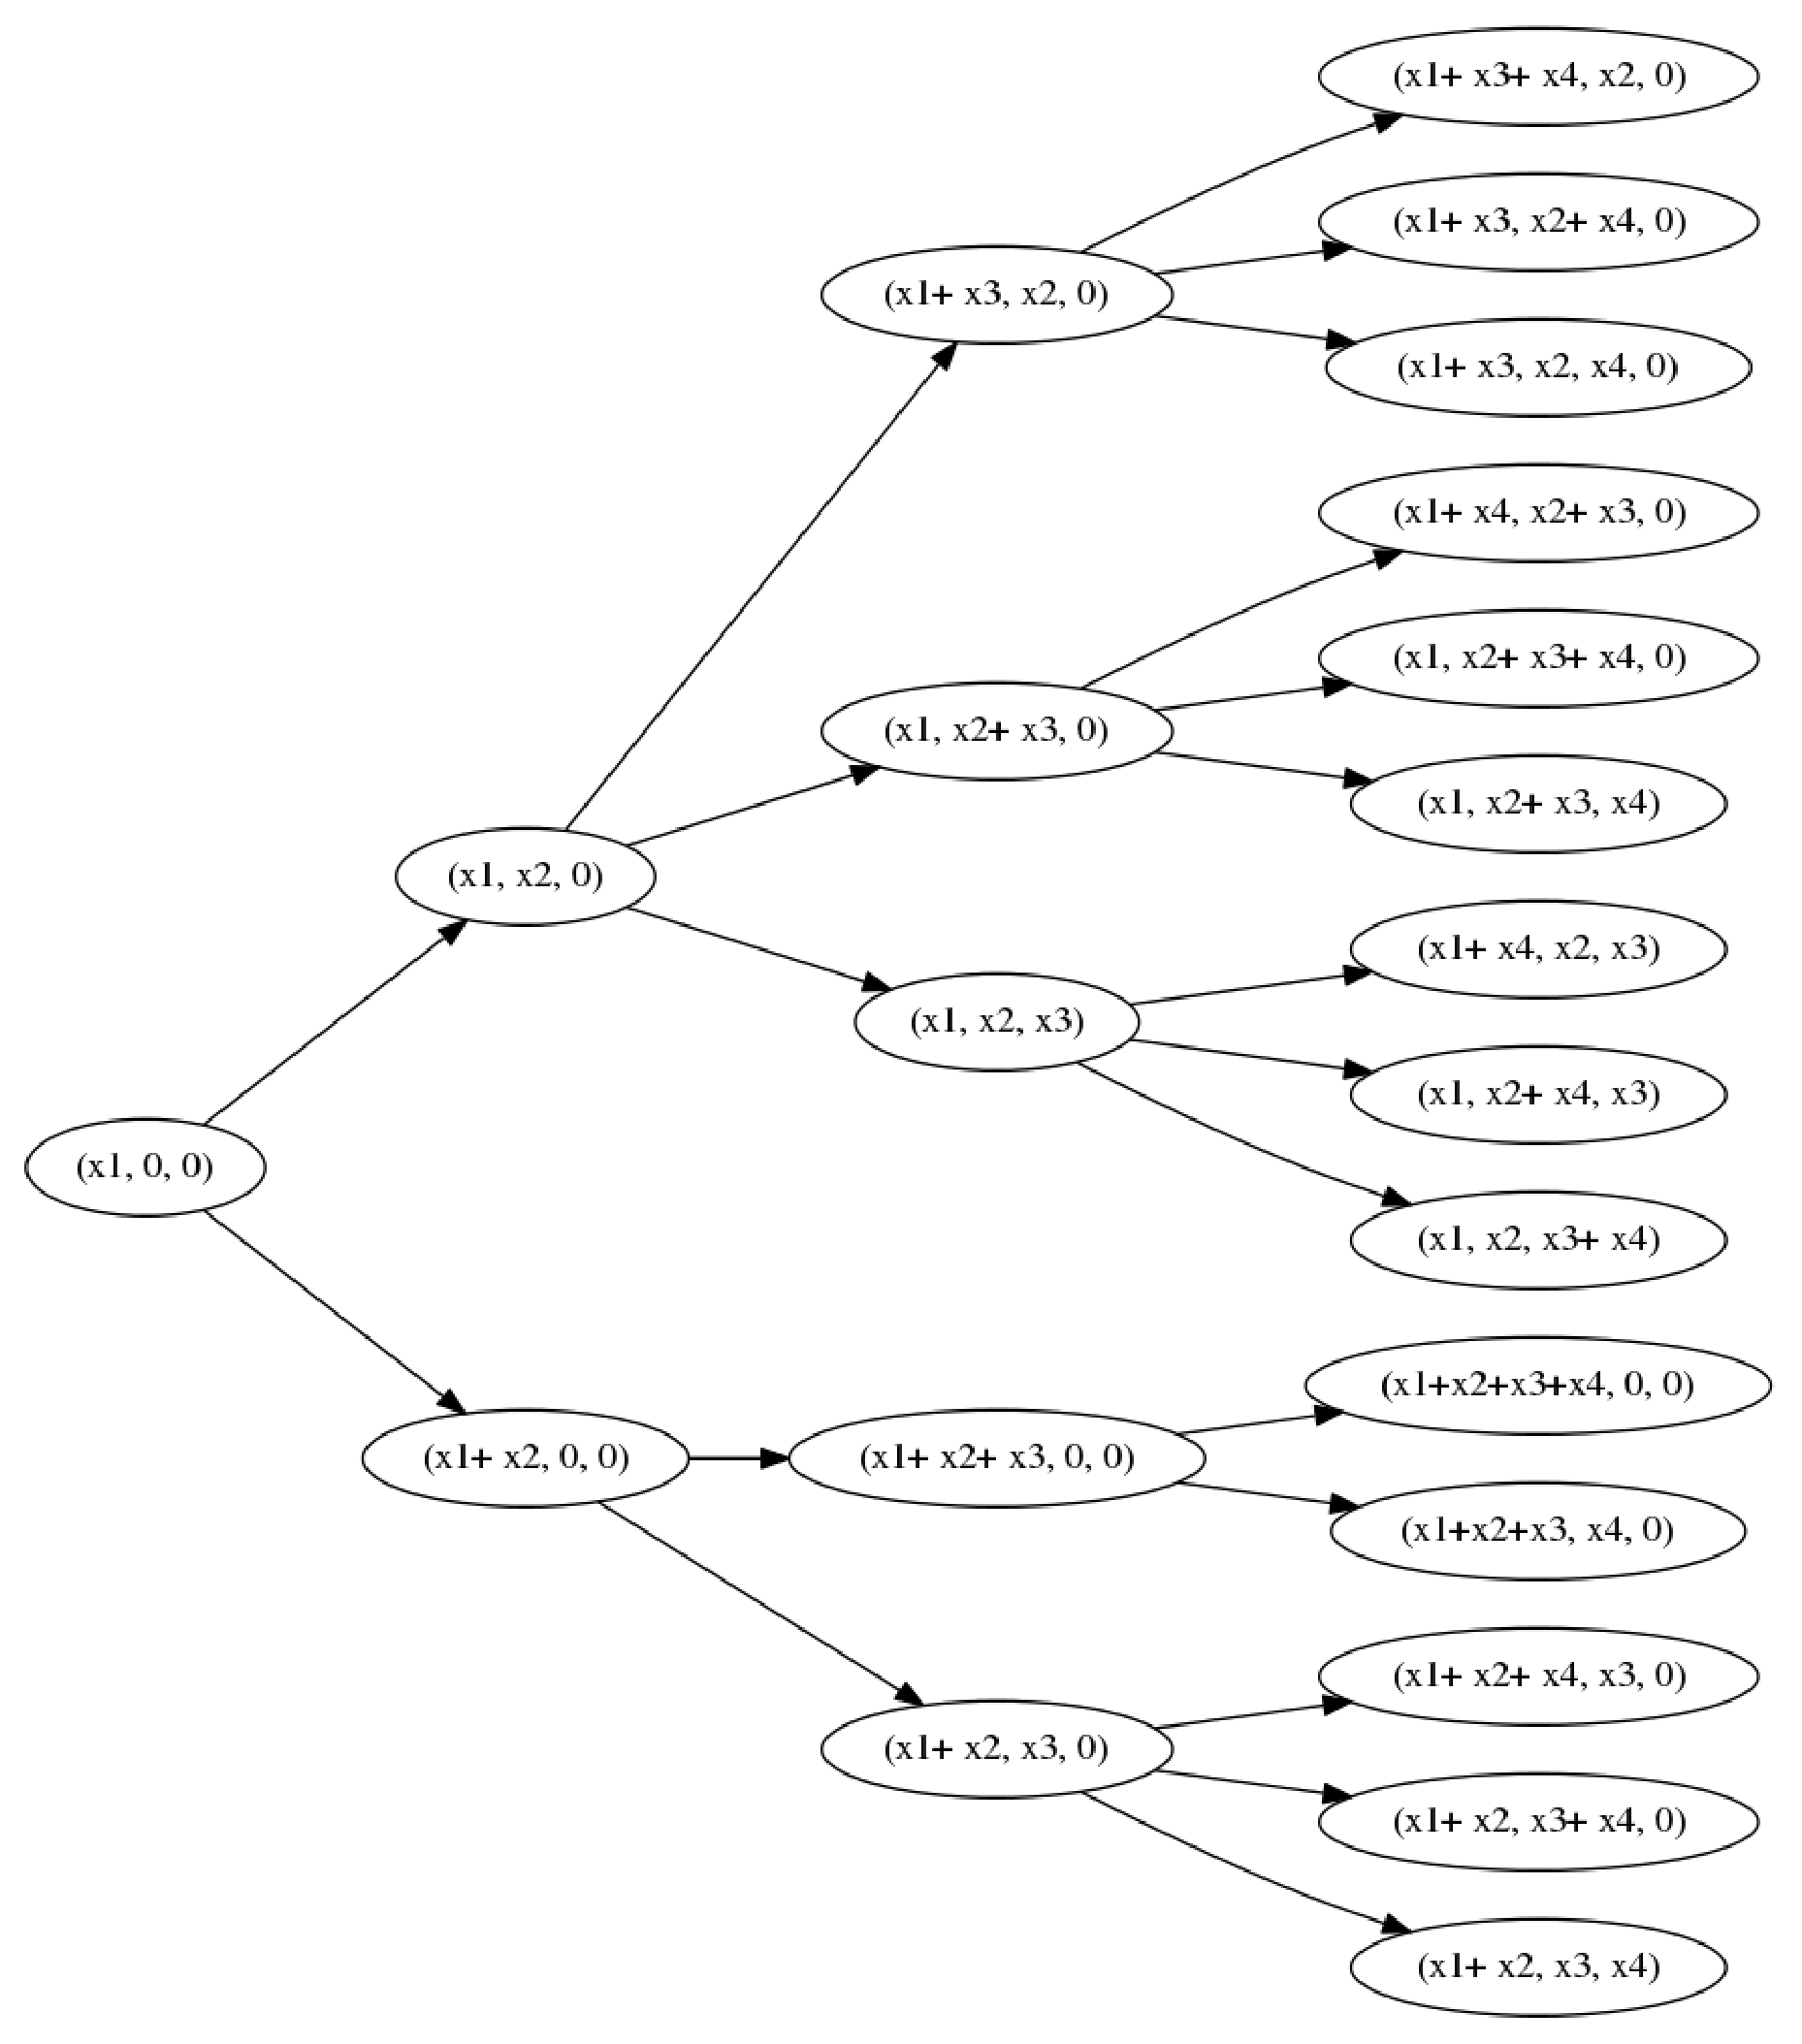
\includegraphics[width= 0.55\linewidth]{./cga3}
	\caption{Exemplo de �rvore de busca ara o (MWNPP): $|S|=4$ e $k=3$}
	\label{figura3}
\end{figure}

Tamb�m parece um m�todo impratic�vel, mas algumas boas ideias ainda podem melhor�-lo.

A maior vantagem das heur�sticas simples, com baixa complexidade, � que elas s�o uma parte importante dos m�todos exatos de enumera��o impl�cita. Uma heur�stica construtiva pode ser aplicada dentro de um algoritmo exato para gerar limites superiores enquanto uma relaxa��o serve para encontrar limites inferiores. Seja $H(I)$ uma heur�stica, $R(I)$ uma relaxa��o e $Opt(I)$ o �timo global para o problema de minimiza��o $I$. Conclui-se que

\begin{equation}\label{equa1}
R(I)\leq Opt(I) \leq H(I)
\end{equation}

Logo, a combina��o inteligente dessas duas coisas pode gerar cortes numa �rvore de busca e acelerar muito um m�todo de enumera��o impl�cita.

Se um valor $R(I)$ constru�do a partir de um n�, $x$, num determinado n�vel da �rvore de busca for maior que o menor dos $H(I)$, corta-se a ramifica��o desse n� por contradi��o com as Inequa��es \ref{equa1} e o mesmo vale para . Esta ideia evita que a �rvore de busca cres�a como na Figura \ref{figura3}.

%-----------------------------------------------------------------------------------------------------------------------------------------
% MODELO DE PROJETO DE QUALIFICA��O DE MESTRADO
%
% CENTRO FEDERAL DE EDUCA��O TECNOL�GICA DE MINAS GERAIS | CEFET-MG
% DEPARTAMENTO DE PESQUISA E P�S-GRADUA��O | DPPG
% AUTOR: LINHA DE PESQUISA EM MODELAGEM, APERFEI�OAMENTO E OTIMIZA��O DE PROCESSOS | MAOP
%
% PARTE: OBJETIVO
%
% ALUNO: Alexandre Frias Faria
%-----------------------------------------------------------------------------------------------------------------------------------------

\chapter{Objetivos e Metodologia} \label{objetivo}
\markboth{Objetivo e Metodologia}{Objetivo e Metodologia}

Este cap�tulo apresenta objetivos gerais, na Se��o \ref{objger}, e espec�ficos, na Se��o \ref{objesp} desse projeto de disserta��o seguido da metodologia empregada, na Se��o \ref{metod}, finalizando com uma breve justificativa, na Se��o \ref{just}.

\section{Objetivos Gerais}\label{objger}

O objetivo geral desse trabalho � o estudo do Problema da k-Parti��o de N�meros e suas solu��es heur�sticas e exatas. 


\section{Objetivos Espec�ficos}\label{objesp}

Os objetivos espec�ficos do presente trabalho � apresentar uma avalia��o da aplica��o de algoritmos heur�sticos com movimentos "gulosos" de troca e realoca��o, testar suas aplicabilidades como limitantes de algoritmos exatos de enumera��o impl�cita e verificar se as heur�sticas propostas geram limites superiores melhores que as da literatura. 

\section{Metodologia}\label{metod}

Para alcan�ar os objetivos, \ref{objger} e \ref{objesp}, usam-se inst�ncias geradas aleatoriamente, como nos poucos trabalhos da literatura, os resultados experimentais finalizar�o a parte de testes da pesquisa. A avalia��o ser� composta por an�lises estat�sticas, compara��es de resultados obtidos na literatura e estrat�gias abordadas nos trabalhos correlatos, citados no Cap�tulo \ref{revisao}.

Para alcan�ar esse objetivo, destaca-se a seguinte sequ�ncia metodol�gica:
\begin{itemize}
	\item[(i)] Finalizar a pesquisa bibliogr�fica sobre o (MWNPP) e sobre as t�cnicas utilizadas para solucion�-lo mesmo em artigos que modificaram o objetivo original do problema.
	\item[(ii)] Verificar outras formas de resolver o (MWNPP) usando algoritmos desenvolvidos para problemas relacionados.
	\item[(iii)] Analisar os resultados obtidos com cada m�todo desenvolvido.
	\item[(iv)] Destacar os resultados de forma comparativa.
\end{itemize}

\section{Justificativa}\label{just}

O (MWNPP) apresenta uma s�rie de algoritmos exatos baseados em m�todos de enumera��o impl�cita e programa��o din�mica. Embora a complexidade desses algoritmos seja exponencial, na pr�tica, eles s�o bem mais r�pidos que o esperado. O mais importante � que um algoritmo que resolva o (MWNPP) em tempo vi�vel pode ser aplicado a outros problemas NP-completos que, geralmente, s�o quest�es auxiliares de problemas reais.
%-----------------------------------------------------------------------------------------------------------------------------------------
% MODELO DE PROJETO DE QUALIFICA��O DE MESTRADO
%
% CENTRO FEDERAL DE EDUCA��O TECNOL�GICA DE MINAS GERAIS | CEFET-MG
% DEPARTAMENTO DE PESQUISA E P�S-GRADUA��O | DPPG
% AUTOR: LINHA DE PESQUISA EM MODELAGEM, APERFEI�OAMENTO E OTIMIZA��O DE PROCESSOS | MAOP
%
% PARTE: CRONOGRAMA DO TRABALHO
%
% ALUNO: Alexandre Frias Faria
%-----------------------------------------------------------------------------------------------------------------------------------------

\chapter{Cronograma do Trabalho} \label{cronograma}
\markboth{Cronograma de Trabalho}{Cronograma de Trabalho}

Neste cap�tulo apresenta-se o cronograma do trabalho explicitando a metodologia adotada at� a conclus�o do mesmo. Listam-se as principais tarefas desde a qualifica��o do projeto at� a defesa da disserta��o.

%-----------------------------------------------------------------------------------------------------------------------------------------
% PERSPECTIVAS
%-----------------------------------------------------------------------------------------------------------------------------------------

\section{Perspectivas} \label{perspectivas}

A tabela \ref{tabelaCronograma} mostra o cronograma do trabalho at� a data prevista para a defesa da disserta��o. Reuni�es com a orienta��o est�o impl�citas.

\begin{table}[h]
	\centering
	\caption{Cronograma do trabalho para o ano de 2016}
	\begin{tabular}{cl}
		\hline		
		\textbf{\small{M�s}}&\textbf{\small{Tarefas}}\\
		\hline
		\small{Junho}&\small{Qualifica��o e finaliza��o da implementa��o e testes}\\
		\small{Julho}&\small{Finaliza��o da disserta��o e marca��o da data da defesa da disserta��o.}\\
		\small{Agosto}&\small{Defesa da disserta��o para obten��o do t�tulo de Mestre.}\\
		\hline
	\end{tabular}
	\label{tabelaCronograma}
\end{table}

Ap�s a qualifica��o do projeto de disserta��o ser� discutida a possibilidade de inclus�o de outras estrat�gia para gerar inst�ncias dif�ceis para o (MWNPP). Em junho, alguns algoritmos j� prontos ser�o codificados para linguagem C++ e comparados. Em julho, os experimentos computacionais finais com inst�ncias dif�ceis geradas aleatoriamente e de outros trabalhos da literatura terminam juntamente com a escrita da disserta��o. A finaliza��o da disserta��o ser� apresentada, inserindo as considera��es finais da orienta��o, e a data da defesa ser� marcada com um m�s de anteced�ncia, conforme solicitado pelo programa. Por fim, em setembro, a defesa da disserta��o para obten��o do t�tulo de Mestre concluir� o presente trabalho.



%-----------------------------------------------------------------------------------------------------------------------------------------
% MODELO DE PROJETO DE QUALIFICA��O DE MESTRADO
%
% CENTRO FEDERAL DE EDUCA��O TECNOL�GICA DE MINAS GERAIS | CEFET-MG
% DEPARTAMENTO DE PESQUISA E P�S-GRADUA��O | DPPG
% AUTOR: LINHA DE PESQUISA EM MODELAGEM, APERFEI�OAMENTO E OTIMIZA��O DE PROCESSOS | MAOP
%
% PARTE: RESULTADOS PRELIMINARES
%
% ALUNO: Alexandre Frias Faria
%-----------------------------------------------------------------------------------------------------------------------------------------

\chapter{Resultados Preliminares} \label{resultados}
\markboth{Resultados Preliminares}{Resultados Preliminares}

\section{Publica��es} \label{publicacoes}

At� o presente momento, este trabalho tem uma publica��o, intitulada, {\em UM ALGORITMO ITERATIVO PARA O PROBLEMA DA K-PARTI��O DE N�MEROS}, publicada no evento CILAMCE-2015 \cite{alexandre:2015}.


\section{Resultados Computacionais} \label{computacionais}

Implementa-se os algoritmos do trabalho em MATLAB vers�o 7. Realizam-se testes em um computador com processador Intel Core i3-M330, 2.13 GHz, 3GB de RAM e sistema operacional Windows 32 bits.

Obtem-se resultados a partir de inst�ncias geradas aleatoriamente. Os conjuntos gerados tem tamanhos entre $100$ e $110$ e os elementos s�o inteiros variando de $50$ at� $350$. O valor �timo do problema - ($opt$), o tamanho do conjunto - $n$ e o n�mero de partes - $k$ s�o par�metros de entrada do gerador de inst�ncias. Um n�mero grande � escrito como soma de outros $k$ n�meros de modo que a diferen�a entre o maior e menor seja igual ao par�metro $opt$. Em seguida, esses $k$ n�meros s�o escritos como soma de outros $\frac{n}{k}$ elementos aleat�rios formando um vetor de tamanho $n$ cuja parti��o �tima tem fun��o objetivo menor ou igual a $opt$. O algoritmo proposto encontrou o �timo exceto nas inst�ncias com valores em negrito.

Abaixo, os resultados dos testes devem ser lidos da seguinte maneira: a vari�vel $si$  indica a i-�sima inst�ncia. O n�mero $k=\{3,4,5\}$ complementa a inst�ncia indicando o tamanho da parti��o. A primeira coluna indica a inst�ncia do experimento. A segunda coluna contem resultados alcan�ados pelo (LPT). A terceira coluna s�o os resultados finais melhorados com o (ILS) partindo do (LPT).

\vspace{2 cm}
\begin{table}[ht!]
\centering

    \begin{tabular}{cccc}
    \hline
    Inst�ncias para k=3         & Algoritmo 1   & Algoritmo 2 & $opt$\\
    \hline
    s1                          & 9             &   3         & 3\\
    s2                          & 51            &   1         & 1\\
    s3                          & 3             &   3         & 3\\
    s4                          & 51            &   3         & 3\\
    s5                          & 39            &   {\bf 10}  & {\bf 4}\\
    s6                          & 49            &   2         & 2\\
    s7                          & 57            &   2         & 2\\
    s8                          & 44            &   5         & 5\\
    s9                          & 3             &   1         & 1\\
    \end{tabular}
\caption{Experimentos demonstrando a melhora provocada pelo (ILS) para k=3}
\end{table}

\newpage

\begin{table}[ht!]
\centering

    \begin{tabular}{cccc}
    \hline
    Inst�ncias para k=4 & Algoritmo 1     & Algoritmo 2 & $opt$\\
    \hline
    s1                          &  41    &    3        & 3\\
    s2                          &  47    &    0        & 0\\
    s3                          &  48    &    5        & 5\\
    s4                          &  50    &    1        & 1\\
    s5                          &  4     &    4        & 4\\
    s6                          &  50    &    {\bf 9}  & {\bf 7}\\
    s7                          &  58    &    0        & 0\\
    s8                          &  48    &    5        & 5\\
    s9                          &  12    &    3        & 3\\
    \end{tabular}
\caption{Experimentos demonstrando a melhora provocada pelo ILS para k=4}
\end{table}

\begin{table}[ht!]
\centering

    \begin{tabular}{cccc}
    \hline
    Inst�ncias para k=5 & Algoritmo 1     & Algoritmo 2 & $opt$\\
    \hline
    s1                          & 16   &   6        & 6\\
    s2                          & 48   &   2        & 2\\
    s3                          & 45   &   6        & 6\\
    s4                          & 49   &   6        & 6\\
    s5                          & 53   &   7        & 7\\
    s6                          & 50   &   0        & 0\\
    s7                          & 62   &   3        & 3\\
    s8                          & 49   &   {\bf 11} & {\bf 6}\\
    s9                          & 51   &   3        & 3\\
    \end{tabular}
\caption{Experimentos demonstrando a melhora provocada pelo ILS para k=5}
\end{table}



\section{An�lise} \label{analise}


Apresentou-se uma proposta de algoritmo heur�stico usando (ILS) com movimentos de realoca��o dos elementos entre as partes para o (MWNPP) na sua vers�o de otimiza��o.  Os resultados obtidos foram testados com inst�ncias geradas aleatoriamente.

O (ILS) empregado com m�todo guloso consegue melhorar a solu��o inicial sempre que esta n�o � �tima. O algoritmo apresentado tem baixa complexidade e atingiu o �timo global em todas as 10 inst�ncias testadas mostrando melhora significativa em rela��o a solu��o inicial constru�da.

Como trabalhos futuros tem-se a melhoria do algoritmo apresentado com uma tabela {\em hash} que melhore a busca pelo movimento de realoca��o, inser��o de um movimentos de permuta entre duas ou mais partes e um quadro comparativo entre os m�todos exatos e aproximados para o problema descrito.






\newpage
\pagestyle{meucabecap}
\newpage

%-----------------------------------------------------------------------------------------------------------------------------------------
% P�S-TEXTUAIS
%-----------------------------------------------------------------------------------------------------------------------------------------

%-----------------------------------------------------------------------------------------------------------------------------------------
% MODELO DE PROJETO DE QUALIFICA��O DE MESTRADO
%
% CENTRO FEDERAL DE EDUCA��O TECNOL�GICA DE MINAS GERAIS | CEFET-MG
% DEPARTAMENTO DE PESQUISA E P�S-GRADUA��O | DPPG
% AUTOR: LINHA DE PESQUISA EM MODELAGEM, APERFEI�OAMENTO E OTIMIZA��O DE PROCESSOS | MAOP
%
% PARTE: REFER�NCIAS
%
% ALUNO: THIAGO MUNIZ STEHLING
%-----------------------------------------------------------------------------------------------------------------------------------------

\addcontentsline{toc}{chapter}{Refer�ncias}
\pagestyle{meucabezz}\markboth{}{}
\markboth{Refer�ncias Bibliogr�ficas}{Refer�ncias Bibliogr�ficas}
\bibliographystyle{PPGEMBST}
%\bibliographystyle{dcu}
\bibliography{refs}

\newpage

\end{document} 